%!TEX root = ../../thesis.tex
%!TEX enableSynctex = true
%*******************************************************************************
%****************************** Third Chapter **********************************
%*******************************************************************************
% **************************** Define Graphics Path **************************
% \ifpdf
%  \graphicspath{{Chapter/tweezers/Figs/Raster/}{Chapter/tweezers/Figs/PDF/}{Chapter/tweezers/Figs/}}
% \else
%  \graphicspath{{Chapter/tweezers/Figs/Vector/}{Chapter/tweezers/Figs/}}
% \fi

\ifpdf{}
    \graphicspath{{Chapters/tweezers/Figs/Raster/}{Chapters/tweezers/Figs/PDF/}{Chapters/tweezers/Figs/}}
\else
    \graphicspath{{Chapters/tweezers/Figs/Vector/}{Chapters/tweezers/Figs/}}
\fi

\chapter[Light-sheet microscopy combined with remote force measurements]{Light-sheet microscopy combined with remote force measurements}\label{chapter:tweezers}
%:\\ \Large Correlating real-time viscoelastic changes with embryonic development}
% \epigraph{\emph{Show me a fish}}{--- Anonymous}
% Section on what we're trying to achieve
%From Julien:
How multicellular organisms enact the morphogenetic programmes that ensure their characteristic forms remains an enigma.
Genetic screens have yielded an array of essential structural, patterning and signalling pathways with which morphogenesis is orchestrated,~\cite{gilbertDevelopmentalBiology2000} however, morphogenesis is ultimately a physical phenomenon that requires a physical explanation.
\emph{In vivo} imaging of morphogenesis allows measurements to be made that reveal stereotypical patterns in the cellular behaviour of individual, and groups of, cells.
These are indicative of active force generation, but are insufficient to construct a quantitative explanation of where forces are generated and how forces propagate within and between tissues.
To overcome these limitations, we require a quantitative characterisation of the physical properties of the tissues involved in order to understand how forces propagate within tissues to bring about morphogenesis.
Measurements of the properties of individual cells,~\cite{mammotoMechanicalControlTissue2010} and of bulk tissues,~\cite{mammotoMechanobiologyDevelopmentalControl2013} have revealed properties typical of both viscoelastic and visco-elasto-plastic solids~\cite{
heisenbergForcesTissueMorphogenesis2013}.
Bulk tissue properties can be estimated using atomic force microscopy to investigate a tissue surface~\cite{serwaneVivoQuantificationSpatially2017}.
Alternatively, micropipette aspiration can probe dissociated cells or explants, however, this method cannot assess deep tissue directly~\cite{maitreAsymmetricDivisionContractile2016,maitreAdhesionFunctionsCell2012}.
More recently, techniques have been developed to measure tissue stress and viscoelastic properties, utilising laser ablation~\cite{bonnetMechanicalStateMaterial2012}, oil droplets~\cite{serwaneVivoQuantificationSpatially2017}, or embedding tissue explants in matrix gel~\cite{zhouForceProductionMechanical2015}.
Most recently, ferrofluid droplets have shown that local tissue properties change with respect to the tissue localisation~\cite{serwaneVivoQuantificationSpatially2017}. %ROX [, in terms of rheological parameters of elasticity and viscosity? Elaborate on these changes.]
There is still a need for methods that can provide a repeated, real-time readout of physical properties and relate those measurements to the underlying morphogenetic behaviour.

A method was developed that can give non-destructive, quantitative measurements of local tissue physical properties at the length scale of a few cells, completed within seconds to minutes, and repeatable over developmentally-significant periods.
To achieve this, biologically-compatible superparamagnetic beads were implanted into developing \gls{zebrafish} embryos and built a four-pole electromagnetic device that produces a controlled magnetic field gradient in 3D, such that a bead can be moved with known force.
Tracking the bead movement gives the dynamic material properties of the surrounding tissue. %ROX  [in terms of elasticity and viscosity? Elaborate on what the system allows you to evaluate.].
This technique was used to study the emergence of the first cohesive tissue of the \gls{zebrafish} blastula, between the “high” to “sphere” stages of development.

It was found that mesenchymal blastomeres become first motile, and then adherent, to form the tissue that will go on to contribute to the first morphogenetic movement of the embryo.
Moreover, there was a three-fold increase in both tissue elasticity and viscosity was associated with the mid-blastula transition.
This was dependent upon E-cadherin-based intercellular adhesions and Rac-1-dependent cell protrusion; abrogating either of these processes interfered with the developmental changes of the embryo.
Interestingly, reducing Rho-kinase-dependent cell contractility increased both tissue viscosity and elasticity and increased the number of cell protrusions.

By using light-sheet microscopy, in conjunction with magnetic tweezers, the fast image of tissue were acquires on a scale large enough to track the topological changes and rearrangement of cells.
The magnitude of change in both of these attributes reduces as tissue elasticity and viscosity increase, and it is evident that the viscoelastic component correlates predominantly to changes in cell morphology, while viscosity dictates the rearrangement of cells.

The work done in this chapter is currently under review with \emph{Nature Materials}
\clearpage

\section{Tissue dynamics in developing organisms}

\subsection{Danio rerio as a developmental model organism}
%From Fran edited
The \gls{zebrafish} (Danio rerio) is a key model organism for vertebrate development.
It shares features of its body plan and developmental stages (\figurename~\ref{fig:zebrafish_stages}) with Xenopus, chickens, and mice~\cite{wolpertPrinciplesDevelopment2006}, indicating the existence of conserved developmental mechanisms.
These mechanisms rely on reproducible, organism-wide patterns of cellular division, migration, death and differentiation during embryonic developmental stages, as well as during adult life.
As this cellular behaviour arises within the context of organism-wide signalling events, a complete understanding of the processes shaping these events requires whole-organism imaging.
Of the vertebrate model organisms, the \gls{zebrafish} is best suited for whole organism imaging from fertilisation until hatching/birth.
The embryo is transparent and small, but can still be physically manipulated, and develops externally from the mother, allowing for imaging uninhibited by surrounding tissue from the parent organism; as a result, \gls{zebrafish} require no atmospheric control to enable growth, unlike cell cultures and other higher order models such as mice.
Moreover, \gls{zebrafish} growth is rapid; a single cell, with a \SI{0.7}{\milli\meter} diameter, becomes a \SI{3.5}{\milli\meter} long larva within three days (see Table~\ref{tab:zfish_dev}).
\gls{zebrafish} are also suitable for genetic studies as the genome is fully sequenced and tools for genetic manipulation are readily available.
Breeding the fish is simple, as sexual maturity occurs at three months after fertilisation, facilitating easy cross-breeding~\cite{kimmelStagesEmbryonicDevelopment1995}.
Finally, the costs of keeping \gls{zebrafish} are lower than that of other vertebrates due to their low space requirements and minimal handler time~\cite{AnimalModelsHuman}.

% The \gls{zebrafish} (\emph{Danio rerio}) is a key model organism for vertebrate development.
% It shares features of its body plan and developmental stages with Xenopus, the chicken, and the mouse \cite{?} (Wolpert et al, 2007)
% , indicating existence of conserved developmental mechanisms of interest.
% These mechanisms rely on organism-wide, reproducible patterns of cellular division, migration, death and differentiation, which occur throughout the organism during development as well as adult life.
% As this cellular behaviour arises within the context of organism-wide signalling events, a truly complete understanding of the processes shaping them requires whole-organism imaging.
% Of the vertebrate model organisms, the \gls{zebrafish} is best suited for whole organism imaging from fertilisation until hatching/birth.
% The embryo is transparent and small, but can still be physically manipulated, and develops outside the mother allowing for imaging uninhibited by surround tissue from the mother; as a result \gls{zebrafish} require no external atmospheres to enable growth, unlike mice.
% \gls{zebrafish} growth is rapid, a single cell of a diameter of 0.7 mm becomes a 3.5 mm-long larva within three days (see Table \ref{tab:zfish_dev}).
% %(see table 1 for overview, Kimmel et al (1995) for detailed description).
% Finally, \gls{zebrafish} are suitable for genetic studies, the genome is fully sequence and there exist tools for genetic manipulation.
% Breeding is simple, sexual maturity occurs at three months post fertilisation making for easy cross-breeding \cite{?} %(D'Costa \& Shepherd, 2009)
% , and the costs of keeping \gls{zebrafish} are lower than that of other vertebrates due to their low space requirements and minimal handler time. \cite{?} (Lieschke \& Currie, 2007).

\begin{figure}
 \centering
 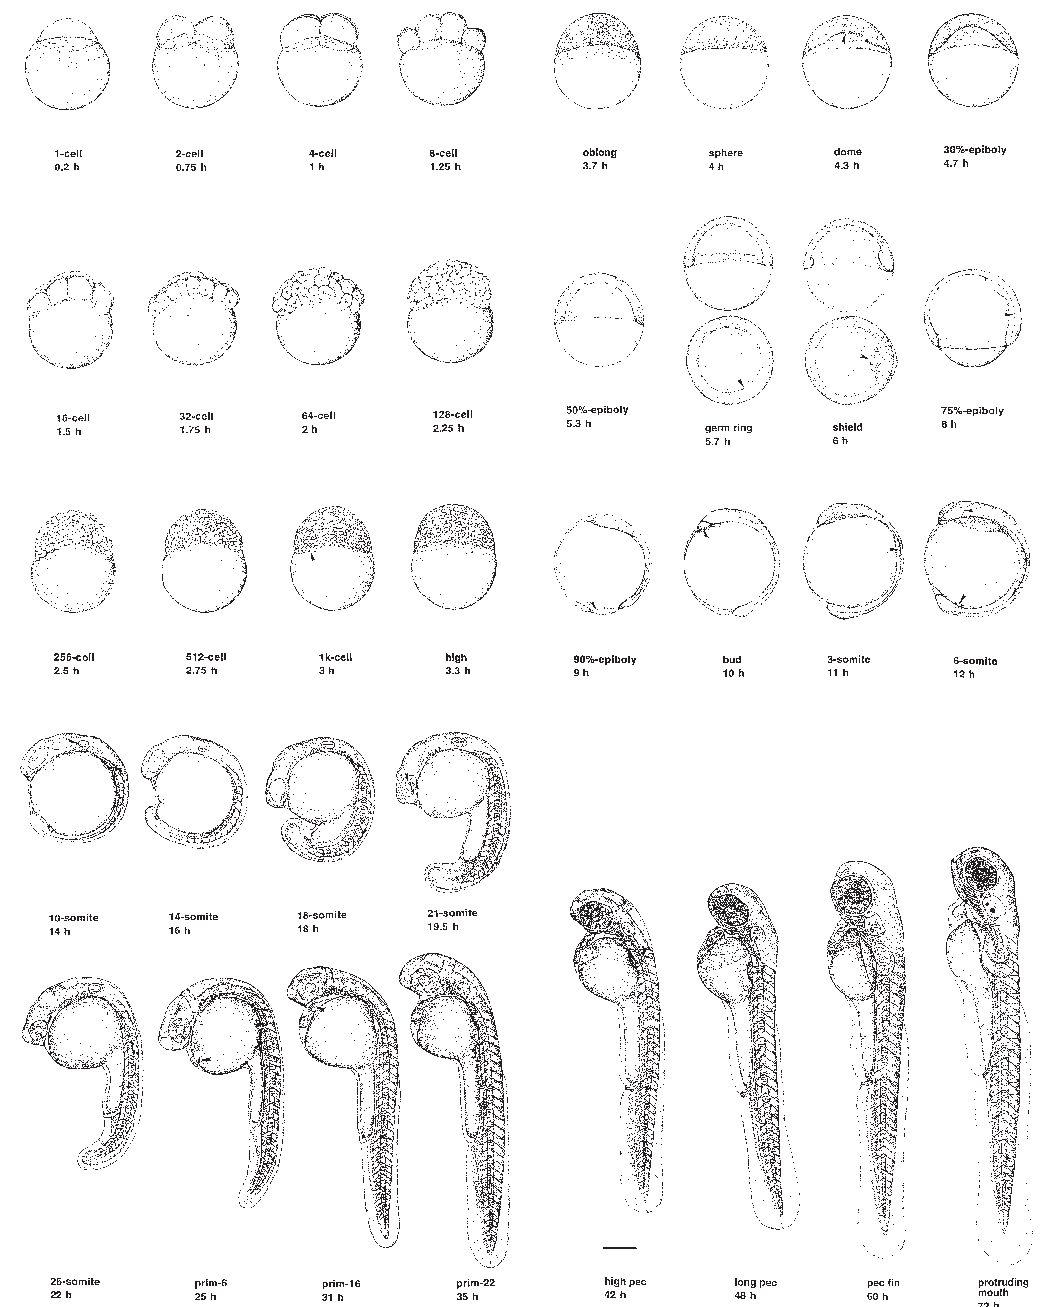
\includegraphics{Chapters/tweezers/Figs/PDF/zebrafish_stages}
 \caption[Periods of embryonal development of the \gls{zebrafish}]{
Periods of embryonal development of the \gls{zebrafish}.
The embryo develops from a single cell into a larva in three days, undergoing extensive morphological changes.
See Table~\ref{tab:zfish_dev}.
 % Periods of embryonal development of the \gls{zebrafish}.
 % The embryo develops from a single cell into a larva in three days, undergoing morphologically apparent changes.
 % See Table~\ref{tab:zfish_dev}.
 }\label{fig:zebrafish_stages}
\end{figure}

\begin{table}
 \centering
 \begin{tabular*}{\textwidth}{rlp{23em}}
 \toprule
 Age / \SI{}{\hour} & Stage & Notes \\
 \midrule
 \SI{0}{\hour} & Zygote & Cytoplasm flows to the animal pole to form the blastodisc.\\
 \SI{0.75}{\hour} & Cleavage & The blastodisc undergoes several rounds of rapid, synchronous, partial cleavage to give 64 blastomeres (and a yolk cell).\\
 \SI{2.25}{\hour} & Blastula & The mid-blastula transition occurs; epiboly begins.\\
 \SI{5.25}{\hour} & Gastrula & More cell migration. Gastrulation, involution, convergence, extension; forming formation of the epiblast and hypoblast.\\
 \SI{10}{\hour} & Segmentation & The tail appears; somites develop; organogenesis starts. \\
 \SI{24}{\hour} & Pharyngula & Circulation begins and pigmentation develops. The body axis straightens. Fins begin development.\\
 \SI{48}{\hour} & Hatching & Primary organ systems complete morphogenesis, cartilage develops, the fish hatches.\\
 \SI{72}{\hour} & Early larva & The swim bladder inflates; food-seeking behaviour occurs. \\
  \bottomrule
 \end{tabular*}
 \caption{Developmental stages of \gls{zebrafish}}\label{tab:zfish_dev}
\end{table}

%Additionally, the \gls{zebrafish} is suitable for genetic studies: its genome sequence and tools for genetic manipulation are available, breeding is easy and possible from three months after fertilisation (D'Costa \& Shepherd, 2009), and the costs of keeping \gls{zebrafish} are low compared with other vertebrates (Lieschke \& Currie, 2007).
%From Fran
%\subsection{Embryonic rheology}
\section{Methods of measuring tissue dynamics}
%\section{Magnetic tweezers combined with Light-sheet microscopy}
%Bit on remote force stuff

The force generation requirements for the investigation of cellular morphogenesis greatly limits which techniques would be suitable for force application and its measurement, as the forces must be applied in the \SIrange{10}{100}{\micro\metre} length scale, of a similar length to the size of a cell.
Furthermore, the magnitude of these forces should be in the \SIrange{10}{100}{\micro\newton} range, of a similar magnitude to the forces that cells are able to generate. %~\cite{}.
It is also desirable for the process to result in minimal heat and light exposure to the organism, as well as to be minimally invasive.
Immediately, common techniques such as mechanical probing, atomic force microscopy, and optical tweezers prove intractable.
Thus, magnetic tweezers were employed in this work as a method of force application and measurement.

Magnetic tweezers operate under the principle of applying a force to a magnetic bead through a magnetic field gradient and are able to apply this force at a distance, without perturbing biological materials, making the technique minimally invasive.
Single-pole tweezer systems, where a single electromagnetic solenoid is able to apply a variable force on a bead in one direction, have been used in a number of experiments to understand the dynamics of cellular force responses~\cite{overbyNovelDynamicRheological2005}.
However, to characterise the force generation in cellular rearrangement fully, it is necessary to generate a magnetic force in an arbitrary direction in three dimensions, as this work demonstrates.
%% Done
%
% The force generation requirements for the investigation of cellular morphogenesis greatly limits which techniques would be suitable for force application and it's measurement: the forces must be applied in the \SI{10}{\micro\meter}-\SI{100}{\micro\meter} length scale, of a similar length to the size of a cell.
% The magnitude of these forces was needed to be in the \SI{100}{\pico\meter} - \SI{100}{\nano\meter} range, of a similar magnitude to the forces that we would expect the cells to be able to generate. \cite{}
% It was also desirable for the process to result in minimal heat and light exposure to the organism, as well as to be minimally invasive.
% Immediately, potentially suitable techniques such as mechanical probing, atomic force microscopy, and optical tweezers prove intractable.
%
% Magnetic tweezers operate under the principle of applying a force to a magnetic bead through a magnetic field gradient and are able apply force at a distance, without perturbing biological materials, making the technique minimally invasive.
% %And so experimental procedures can be designed so that the process is minimally invasive to the organism, which is highly desirable for this particular application.
% %By using a bead
% %By choosing a suitable magnetic material for the bead, and designing the electromagnets appropriately, magnetic tweezers are also able to generate the required force range at the required length scales.
% Single-pole tweezer systems, where a single electromagnetic solenoid is able to apply a variable force on a bead in one direction, have been used in a number of experiments to understand the dynamics of cellular force responses. \cite{}
% However, to fully characterise the force-generation in cellular rearrangement, it is necessary to generate a magnetic force in an arbitrary direction in three dimensions.

%Magnetic tweezers are able to apply a remote force on a magnetic probe through tissue.
%Several other techniques exist to probe
%TODO Talk about direct tissue probing using AFM or Optical tweezer

\subsection{Magnetic tweezers}
%% Fix

The design of the magnetic tweezers was based on a previously published design~\cite{vicci3DMagneticForce2003}, which is compatible with large samples, such as the \gls{zebrafish} embryo employed in this work; and was shown to generate sufficient forces using COMSOL simulations.
This section presents the development of the magnetic tweezers including the imaging chamber required by the \gls{LSFM}.
The mechanical design of the magnetic tweezers was based on a monopole model.
In this simplification the magnetic field is assumed to be generated by point sources (monopoles) around a sample containing a magnetic bead.
The sum of the aggregated monopole strengths must equal zero because, in nature, there are no actual sources or sinks of magnetic flux (i.e.~solenoids generate dipole magnetisation).
In this model, a force acting on the bead in the direction of a monopole can be approximated by~\cite{jacksonClassicalElectrodynamics1998,amblardMagneticManipulatorStudying1996}.
The magnetic dipole moment, \(\mathbf{m}\), induced in the bead by a magnetic field, \(B\), is given by:

\begin{align}
\textbf{m} = \frac{\pi d^3 }{2 \mu_0} \frac{\mu_r -1}{\mu_r +2} \mathbf{B}
\intertext{A force, proportional to the magnetic dipole moment, is then exerted on the bead in the presence of magnetic field gradients:}
\mathbf{F} = \frac{\pi d^3 }{2 \mu_0} \frac{\mu_r -1}{\mu_r +2} \mathbf{\nabla} \mathbf{B}^2
\end{align}

Where \(d\) is the diameter of the bead, \(\mu_0\) is the magnetic permeability of free space, \(\mu_r\) is the relative magnetic permeability of the bead and \(\mathbf{B}\) is the magnitude of the field generated by a magnetic monopole.
\(\mathbf{B}\) is in the form of \(\frac{B_p}{r^2}\) where \(B_p\) is the monopole strength and \(r\) is the distance from the monopole.
Hence the gradient \(\nabla \mathbf{B}\) of the field is \(2 \frac{B_p}{r^3}\), and the force on the bead proportional to \(2\frac{B_{p}^2}{r^5}\)~\cite{vicci3DMagneticForce2003}.
In the mechanical design of the magnetic tweezers, it was thus desirable to position magnetic poles as close as possible to a sample.

A minimum of four monopoles is required to achieve effective 3D specification of the force acting on the bead.
The optimal configuration is a tetrahedral geometry, where monopoles are distributed on the vertices of a tetrahedron.
Deviation from this geometry limits the range and directionality of achievable forces.
Finally, only a single bead should be used at a time, as agglomeration of beads influences the magnetic field distribution due to the interactions between the beads, and thus disturbs the monopole model~\cite{bauschMeasurementLocalViscoelasticity1999}.
The magnitudes and gradients of the magneticfield in the space between the poles is controlled by four solenoid coils; by varying the currents in these coils independently, one may control the the magnitude and direction and magnitude of the force acting on the bead.

\subsubsection{Model Theory}

\begin{figure}
 \centering
 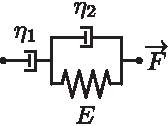
\includegraphics{Chapters/tweezers/Figs/PDF/viscoelastic_model}
 \caption[Viscoelastic model for embryonic tissue]{
 Viscoelastic model for embryonic tissue used in this work; consisting of a dash-pot in series with a dash-pot and spring in parallel.
 The spring, \gls{E_visc}, represents the stiffness of the ensemble tissue, the first dash-pot (\gls{eta_1_visc}) represents tissue viscosity and the second dash-pot (\gls{eta_2_visc}) represents cellular viscosity.
 %
 % Viscoelastic model used for embryonic tissue used in this work; consisting of a dash-pot in series with a dash-pot and spring in parallel.
 % The spring (\gls{E_visc}) represents the stiffness of the ensemble tissue, the first dash-pot (\gls{eta_1_visc}) represents tissue viscosity and the second dashpot (\(\eta_2\)) represents cellular viscosity.
 }\label{fig:viscoelastic_model}
\end{figure}

The simplest phenomenological model capable of mimicking the viscoelastic response of a developmentally early \gls{zebrafish} embryo, subject to strain generated by a moving, spherical, rigid object, is a one‐dimensional linear combination of an elastic spring and viscous dash‐pots.
More precisely, the model assumes a parallel spring and dash‐pot~\cite{meyersMechanicalBehaviorMaterials2008} in series with a second dash‐pot, see \figurename~\ref{fig:viscoelastic_model}.

The model is described by the following parameters: dynamic viscosities, \gls{eta_1_visc} and \gls{eta_2_visc}, and elastic stiffness, \gls{E_visc}.
When a strain \(\sigma \) is applied, the spherical rigid object, in this case a magnetic bead made of superparamagnetic nanoparticles embedded into a polyester matrix, moves and the displacement is quantified by the strain \(\epsilon \).
The same parameter is used to evaluate the recovery phase, when \(\epsilon = 0\).
The experimental protocol used here consists of two phases: the creep phase, where from equilibrium the state at \(t=0\) an instantaneous and constant force is applied on the bead and kept for a given time, \(t_1 \) (\SI{60}{\second}); and the recovery phase where the force is removed at \(t_1\) where the bead displacement is monitored for a suitable time period (\SI{120}{\second}).
To model the equations of motion the a linear spring is described by:
%to derive the model's equations, we recall the viscoelasticity’s fundamental equations. A linear spring is described by:

\begin{align}
 \epsilon &= \frac{1}{\gls{E_visc}} \sigma \label{eq:linearspring}
 \intertext{while a dash-pot obeys:}
 \dot{\epsilon} &= \frac{1}{\eta}\sigma
 \intertext{The equation for a spring and a dash-pot connected in parallel follows as:}
 \sigma = \sigma_E + \sigma_{\eta_{2}} &= E \epsilon_p + \eta_{2} \dot{\epsilon_p}\\
 \ln\left(\frac{\sigma}{\eta_{2}}-\frac{E}{\eta_2} \epsilon_p \right) &= -\frac{E}{\eta_{2}}t+\ln C_1
 \intertext{Setting the initial conditions of \(\epsilon_p = 0\) at \(t = 0\):}
 \epsilon_p &= \frac{\sigma}{E}\left(1-\exp\left(-\frac{E}{\eta_2}t\right)\right)
 \intertext{The temporal variation of the dash-pot is ruled by:}
 \sigma = \eta_1 \dot{\epsilon_s} &\implies \epsilon_s = \frac{\sigma}{\eta_1}t
 \intertext{Knowing that \(\epsilon = \epsilon_s + \epsilon_p\), the strain variance is therefore:}
 \epsilon &= \frac{\sigma}{\eta_1}t + \frac{\sigma}{E}\left(1-\exp\left(-\frac{E}{\eta_2}t\right)\right)
\end{align}
\begin{align}
 \intertext{During the second phase, which starts at \(t_1\), the force is no longer applied %\(\sigma = 0\)
 and the total strain is given by the
 previous displacement of \(\eta_1\) dash‐pot blocked at \(t = t_1\), and the relaxation of the Kelvin‐Voigt model which is described by:}
 E \epsilon_p + \eta_2 \dot{\epsilon_p} = 0 \implies \epsilon_p = C_2 \exp\left(-\frac{E}{\eta_2}t\right)
 \intertext{From the continuity of strain and \(t = t_1\), \(C_2\) becomes:}
 \frac{\sigma}{\eta_1}t + \frac{\sigma}{E}\left(1-\exp\left(-\frac{E}{\eta_2}t_1\right)\right) = C_2 \exp\left(-\frac{E}{\eta_2}t\right)\\
 C_2 = \frac{\sigma}{E}\left(\exp\left( \frac{E}{\eta_2}t_1\right)-1\right)
 \intertext{So, for \(t \geq t_1\), the strain is:}
 \epsilon = \frac{\sigma}{\eta_1}t_1 + \frac{\sigma}{E}\left(\exp\left( \frac{E}{\eta_2}t_1\right)-1\right)\exp\left(-\frac{E}{\eta_2}t\right)
\intertext{The equations of motion may be summarised as}
 \epsilon =
 \begin{cases}
 \frac{\sigma}{\eta_1}t + \frac{\sigma}{E}\left(1-\exp(-\frac{t}{\tau_2})\right) &\text{for } t\geq t_1\\
 \frac{\sigma}{\eta_1}t_1 + \frac{\sigma}{E}\left(\exp\left( \frac{t_1}{\tau_2}\right)-1\right)\exp\left(-\frac{t}{\tau_2} \right) &\text{for } t\leq t_1
 \end{cases} \label{eq:modelfitting}
 \intertext{ where \(\tau_2 = \frac{\eta_2}{E}\) } \nonumber
\end{align}

%The parameters from \eqref{eq:modelfitting} need to be reviewed and amended if one intends to link them to experimental data as one applies a known force and looks at the displacement of the bead from its initial position and not to stress and strain.

A bead moving through a viscous fluid can be described by Stokes' law \(F = 6 \pi \eta' r \nu \), where \(r\) is the radius of the bead and \(\nu \) is the critical velocity of the bead.
Stokes' law may be written as:

\begin{align}
 F &= 6 \pi \eta' r \frac{dx}{dt} \\
 \implies \frac{F}{\pi r^2} &= 6 \eta' \frac{d}{dt}\frac{x}{r} \\
 \implies \sigma &= 6 \eta' \frac{\epsilon}{dt}
 \intertext{Giving the equation of a dash-pot}
 \dot{\epsilon} = \frac{\sigma}{\eta}
\end{align}

To model the elastic spring, the elastic response of the tissue due to the bead displacement is approximated by the Thomson's solution of a point force in an infinite isotropic medium~\cite{l.d.landaue.m.lifshitzTheoryElasticity1970}.
The displacement (\(\mathbf{u}\)) in cylindrical coordinates (\((p,z)\)) for a point force (\(F_z\)) located at the origin and directed along the (\(z\)) axis is given by:

\begin{align}
 \mathbf{u} = \frac{F_z}{4 \pi \mu r }\left[ \frac{pz}{4(1-v)r^2} \mathbf{\hat{p}}+\left(1- \frac{p^2}{4(1-v)r^2}\right)\mathbf{\hat{z}}\right]\label{eq:thomsons}
\end{align}

Where \(\mathbf{\hat{p}}\) and \(\mathbf{\hat{z}}\) are unit vectors, \(\mu \) is the shear modulus (deformation at constant volume) and \(\nu \) is Poisson's ratio (a negative ratio of transverse to axial strain of a specimen, under an axial force).
As only forces in the \(\mathbf{\hat{z}}\) direction are being considering, Equation~\eqref{eq:thomsons} becomes:

\begin{align}
 u_z &= \frac{F_z}{4 \pi \mu r }\left[\left(1- \frac{p^2}{4(1-v)r^2}\right)\right]
 \intertext{Evaluating the displacement only on the \(z\) axis where \(p=0\), reduces this to:}
 \nabla z &= \frac{F_z}{4\pi \mu r}
 \intertext{In the close proximity to the bead of radius \(r_{\text{bead}} \), the displacement is given by:}
 \frac{\nabla z}{r_{\text{bead}}} = \frac{1}{4 \mu} \frac{F_z}{\pi r_{\text{bead}}^2} & \implies \epsilon = \frac{1}{4\mu} \sigma
\end{align}
Which is equivalent to~\eqref{eq:linearspring} when substituting \(E \) with \(4\mu \).

\subsection{Magnetic tweezer design}

In the magnetic tweezer systems a square loop of iron was used to carry magnetic flux from four solenoids to four embedded magnetic tips.
The lower magnetic tips were mounted azimuthally at \SI{30}{\degree}, allowing for the very large \SI{1.1}{\text{NA}}, long working distance, Nikon, objective lens to image the magnetic centre of the magnetic poles.
However, this allowance for the large objective lens by re-orientating the tweezer poles reduces the the maximum magnetic field strength by \SI{10}{\percent}.
Orienting the poles at the optimal angle to the azimuth (\SI{45}{\degree}) would provide \SI{2.33}{\tesla} from COMSOl simulations.

\begin{figure}
 \centering
 \begin{subfigure}[t]{0.45\linewidth}
  \centering
  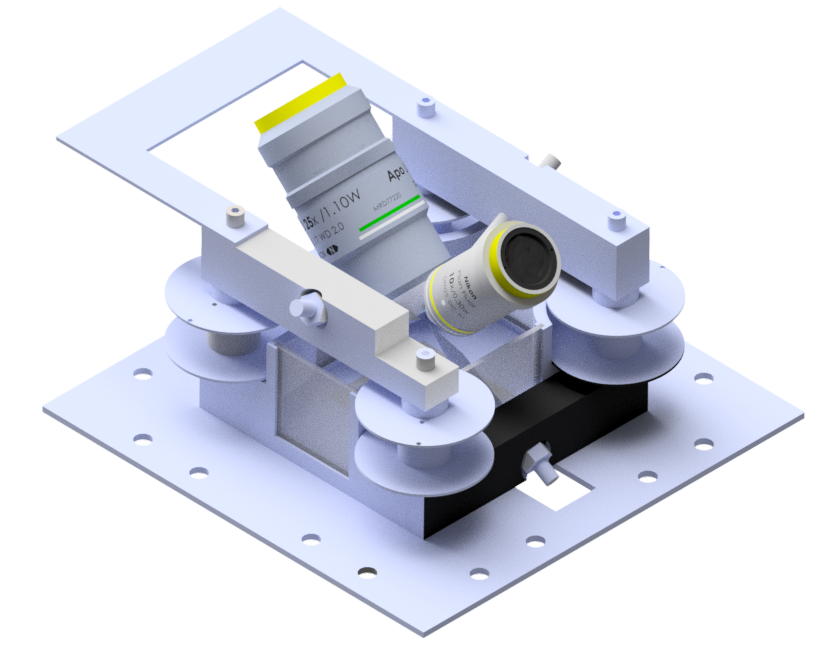
\includegraphics[width=\linewidth]{tweezer_spim_render_shooped}
  \caption{\Gls{light-sheet} objective lens placed within the magnetic tweezer chamber.}
 \end{subfigure}\quad
 \begin{subfigure}[t]{0.45\linewidth}
  \centering
  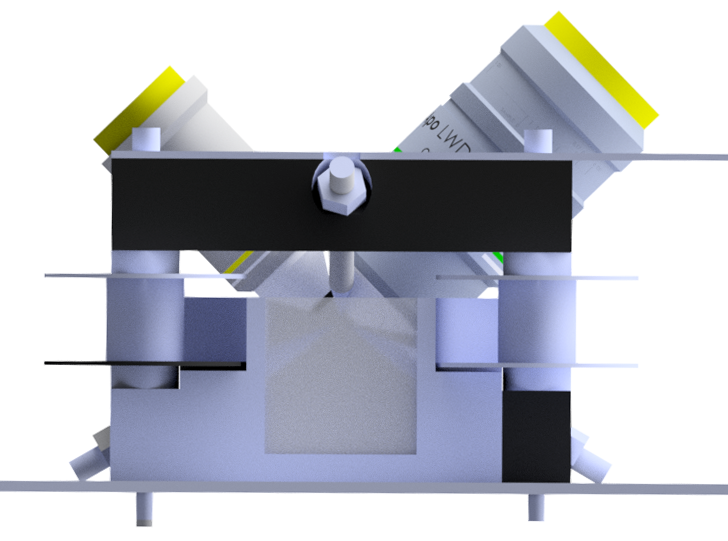
\includegraphics[width=\linewidth]{tweezer_spim_render_side}
  \caption{Side view with magnetic centre of tweezers at the double focus of the illumination and imaging objective lenses.}
 \end{subfigure}
 \caption{CAD designs of the magnetic tweezer housing coupled to the light-sheet objective lenses.}\label{fig:tweezer_spim}
\end{figure}
%\subsubsection{Mechanics}
% Fitting objectives in
% Keeping fish alive
%\subsubsection{Simulations}
\subsubsection{Imaging chamber design}

The imaging chamber presented in \figurename~\ref{fig:fep_chamber} was 3D printed with \gls{ABS} to allow for modular and rapid re-design.
Clear acrylic windows were added to allow for a positioning camera (PiCam) to be placed below the tweezer system, as seen in \figurename~\ref{fig:tweezer_spim}b, which aided with the positioning of the \gls{zebrafish}.
The chamber was watertight and featured heating pads to maintain the embryo medium and zebrafish at \SI{28.5}{\celsius} during imaging.

% The imaging chamber presented was 3D printed in ABS (Acrylonitrile butadiene styrene) to allow for modular and rapid re-design.
% Clear acrylic windows were added to allow for a positioning camera (PiCam) to be placed below the tweezer system, this aided with the positioning of the \gls{zebrafish}.
% The chamber was water tight and featured heating pads to maintain the embryo medium and \gls{zebrafish} at a comfortable during imaging.

\begin{figure}
 \centering
 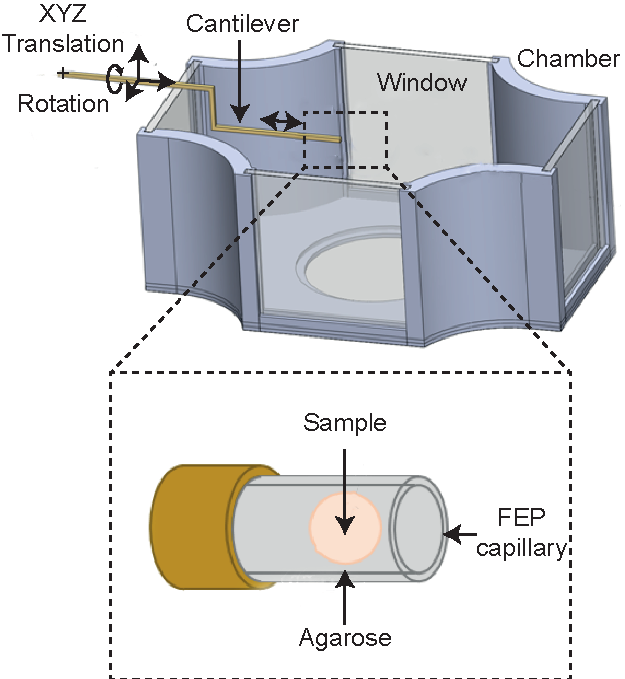
\includegraphics{Chapters/tweezers/Figs/PDF/fep_chamber}
 \caption{3D printed chamber for housing the magnetic tweezers whilst providing ambient living conditions for a developing \gls{zebrafish}.}\label{fig:fep_chamber}
\end{figure}

%Contraints specifications and requirements
\subsubsection{Force calibration}

The 3D magnetic field gradient generated by the quadrupole was shaped by a combination of currents to obtain forces in the range of \SI{8}{\nano\newton}.
Force calibration was realised by analysing the velocities of a \SI{41.17}{\micro\metre} diameter paramagnetic bead in silicone oil of known viscosity at different combinations of intensities of currents.
The coordinate systems of the magnetic tweezers and the light-sheet system had to be aligned due to the non-linear decline of force of the magnetic field away from the magnetic centre.
This was achieved by defining an origin within the tweezer system itself, where force in every direction was maximal.
This point was then recorded by inserting a fiducial magnetic bead, which was attached to an arm and positioned using micrometer screws.
Once the tweezer system was fixed to the light-sheet system, the automated stage was driven such that the fiducial bead was at the imaging centre of the camera and at the axial centre of the piezo objective actuator.
The tweezer positioning was coarse-positioned by eye using the automated stage, followed by fine correction utilising the bright-field imaging built into the sample chamber.

% 3D magnetic field gradient is shaped by a combination of currents to obtain forces of range of .
% Force calibration was realised by analysing the velocities of a diameter paramagnetic bead in known viscosity silicone oil at different combination of intensities of currents.
% The coordinate systems of the Magnetic tweezers and the light-sheet system were required to be aligned due to the non-linear decline of force of the magnetic field away from the magnetic centre.
% This was achieved by defining an origin within the tweezer system itself, where force in every direction was maximal.
% This point was then recorded by carefully inserting a fiducial magnetic bead attached to an arm and positioned using micrometer screws.
% Once the tweezer system was fixed to the light-sheet system, the automated stage was carefully driven such that the fiducial bead was at the imaging centre of the camera and the axial centre of the Piezo objective actuator.
% The tweezer positioning was coarse positioned by eye using the automated stage, fine correction followed by utilising the bright-field imaging built into the sample chamber.

\subsubsection{Synchronisation}

The magnetic tweezers were calibrated and automated using current amplifiers driven by voltages from a Raspberry Pi.
Simple \gls{RS232} commands controlled the amount of force, the direction and the on/off state of the tweezers.
These commands were then sent from the \gls{LabVIEW} controller of the \gls{light-sheet} system to ensure good synchronisation between the initial drive of the bead and the start of the volume acquisition.
%
% The magnetic tweezers were calibrated and automated using current amplifiers driven by voltages from a Raspberry Pi.
% Simple RS232 commands could control the amount of force, direction and on/off state of the tweezers.
% These commands were then sent from the LabVIEW controller controlling the light-sheet system to ensure good synchronisation between the initial drive of the bead and the start of the volume acquisition.

\subsection{Biological methodology}

Zebrafish embryos were harvested immediately after fertilisation and incubated at \SI{28.5}{\celsius}.
Embryo lines that were used were: wild-type (WT), Tg~(beta-actin:mCherry-CAAX) (labelling membranes), Tg~(beta-actin:Lifeact-eGFP) (labelling F-actin) and Tg~(beta-actin:Myosin2- mCherry) (labelling myosin).
Transplantations were performed at 1k-cell stage using a tip broken elongated capillary mounted on an oil-filled pressurised system controlled by a syringe.
Beads, or cells, were transplanted at 1k-cell stage.
Beads were incubated in \SI{4}{\percent} BSA for \SI{10}{\minute} at \SI{28.5}{\celsius} before injecting to reduce the chances of bead rejection from the embryo.
% Transplantations were at 1k-cell stage using a tip broken elongated capillary~\cite{} mounted on an oil filled pressurised system controlled by a syringe \cite{}.
% Beads were incubated in 4\% BSA before grafting to reduce chances of bead rejection when injected and were transplanted at 1k-cell stage.

The soft egg sack was removed from around the \gls{zebrafish} embryo (the \gls{chorion}) which, if left on, would degrade the optical imaging.
A stereo-microscope was used so dechorionation could be done by eye with careful and precise use of very sharp tweezers.
This was done in warm embryo medium on a bed of \SI{1}{\percent} agarose because exposed embryos will rupture on contact glass.
The dechorionated embryos were pipetted into warm low melting point agarose and then immediately drawn up into a length of \gls{FEP} tubing.

\subsubsection{Analysis}

All tests were performed with R software.
A linear mixed effect model was performed to compare rheological parameter trends in different loss-of-function assays.
Anova tests compared linear fits on developmental trends of the rheological parameters between \gls{WT} and loss-of-function conditions (mutants).
The percentage bend correlation method was used for correlation between cell and rheological parameters to take outliers into account~\cite{wilcoxPercentageBendCorrelation1994}. %ROX [can you reference these methods?]

% \subsection{Biological methodology}
% Embryos were harvested just after fertilisation and incubated at \SI{28.5}{\celsius}.
% Embryo lines used were: wild types (WT), Tg(beta-actin:mCherry-CAAX) (labelling membranes), Tg(beta-actin:Lifeact-eGFP) (labelling F-actin) and Tg(beta-actin:Myosin2-mCherry).
% \subsubsection{Bead and cell transplantation}
%
% Transplantations were performed at 1k-cell stage using a tip broken elongated capillary [] mounted on an oil-filled pressurised system controlled by a syringe []. Beads, or cells, were transplanted at 1k-cell stage. Beads were incubated in 4% BSA [time, temperature] before grafting [grafting to what?] to reduce the chances of bead rejection when injected into the embryo.
%
% \subsubsection{Bead and cell transplantation}

\section{Algorithmic bead tracking}

To perform a model fitting, as derived in Equation~\eqref{eq:modelfitting}, the magnetic bead was tracked algorithmically.
Each volume was \SI{2048 x 2048 x 100}{}~\text{voxels}, with each volume acquisition taking \SI{5}{\second}.
Each push-pull experiment produced 42 volumetric spatial coordinates in time (\(x,y,z,t)\), hence the entire data set to be analysed was \SI{172}{\giga\byte}.
Two methods of bead tracking were explored, slice-wise Hough transform analysis and template matching.
%
% To perform a model fitting as derived in \eqref{eq:modelfitting} the magnetic bead needed to be tracked algorithmically.
% Each volume was \(2048 \times 2048 \times 100\) voxels, with each volume acquisition taking 5 seconds.
% Each push-pull experiment produced 42 x,y,z spatial coordinates in time, hence the entire data set to be analysed was 172 GB.
% Two methods of bead tracking were explored, slice-wise Hough transform analysis and template matching.

\subsection{Hough-based bead tracking}

The Hough transform is a feature-tracking mechanism used to transform an image into a space whereby intensity minima or maxima represent circles.
These localised maxima correspond to multiple circles in the image space of a given range of radii as provided to the function.
In the analysis employed here, the first iteration of the analysis algorithm exhaustively searched for circles, with varying threshold sensitivity, until a single circle (of the correct radius through the image volume) was found.
Once singular circles were found slice-wise, a circle was fit to the radii found in each slice to localise the sphere in \(z\).
This lead to multiple computationally expensive transforms being applied and the algorithm being slow.
It is possible to use a 3D Hough transform that searches for spheres rather than circles; again, multiple matches are likely to be returned, resulting in tracking errors.
% The Hough transform is a featuring tracking mechanism used to transform an image into a space whereby intensity minima or maxima represent circles.
% These localised maxima then correspond to multiple circles in the image space of a given range of radii as provided to the function.
% The first iteration of the analysis algorithm would exhaustively search for circles with varying threshold sensitivity until a single circle was found of the correct radius through the image volume.
% Once singular circles were found slice-wise, a circle was fit to the radii found in each slice to localise the sphere in \(z\).
% This lead to multiple computational expensive transforms being applied and the algorithm being slow.
% It is possible to use 3D Hough transform that searches for spheres rather than circles; again, multiple matches are likely to be returned resulting tracking errors.

\subsection{Template matching}

As only a single sphere could be found in each image volume, a template-matching approach was explored.
Initially, an ideal bead was extracted from an image volume for future analyses (see \figurename~\ref{fig:bead_correlation}).
However, it was found empirically that the ideal bead volume template was more likely to chase cells than an artificially, computed, idealised bead.
To construct a virtual bead, a virtual volume was constructed and a white, hollow sphere of the correct pixel radius (\SI{160}{\text{px}}) was superimposed.
%
%
% As only a single sphere could be found in each image volume, a template-matching approach as explored.
% Initially an \emph{ideal bead} was extracted from an image volume for future analyses (see Figure \ref{fig:bead_correlation}).
% However, it was found empirically that the ideal bead volume was more likely to chase cells more so than a virtual idealised bead.
% To construct a virtual bead, a virtual volume would be constructed and a white hollow sphere of the correct pixel radius (160 px) would be superimposed.

Template matching techniques fundamentally rely on the cross-correlation of two images or volumes.
Cross-correlation is made programmatically quicker by operating in Fourier space for convolution rather than iteratively in image space.
Although this does decrease the overall computation time, the net memory usage of the algorithm increases.
As such, care has to be taken to avoid \gls{RAM} overfilling, as this can cause the algorithm to crash;
particularly in operating systems without a well-managed swap-space; or cause the swap- space to be used, slowing the algorithm as it reads large Fourier space volumes off of a slower hard-drive.

% Templating matching techniques fundamentally rely on the cross-correlation of two images or volumes.
% Cross-correlation is made programmatically quicker by operating in Fourier space for convolution rather than iteratively in image space.
% Though this does decrease the overall computation time, the overall memory usage of the algorithm will increase.
% As such care has to be taken to avoid Random Access Memory (RAM) overfilling as this can either cause the algorithm to crash.
% Particularly in operating systems without a well managed swap-space; or, the swap-space is used and the algorithm becomes very slow as it reads large Fourier space volumes on and off of a slower hard-drive.

To circumvent large amounts of memory being used, a windowing technique	was employed to ensure that the minimal amount of voxels was needed for analysis.
The cuboidal window was set to be twice the pixel radius of the bead in each dimension which was arbitrarily set with the assumption that the bead would not move out of the window between two concurrent time points.
Between each frame, the centre of the window was shifted to be aligned with the centre of the bead.
The voxels within this window were analysed and the window shifted again by the relevant offset.
The bead centres were then exported, in 3D, to a text file for further analysis.

% To circumvent large amounts of memory being used a windowing technique was employed to ensure a minimal amount of voxels needed were being analysed.
% The cuboidal window was set to be double the radius in each dimension, this was arbitrarily set with the assumption that the bead would not move out of the window between concurrent two time points.
% Between each frame the centre of the window would be shifted to be aligned with the centre of the bead.
% The voxels within this window were analysed and the window shifted again by the relevant offset.
% The bead centres in 3D were then exported to a text file for analysis.

The seed location, in the first frame for the bead, was found in one of two ways.
A best guess of bead location was found by downsampling the resolution of the image stack and performing a template match on the stack, after which a finer search was performed, and the algorithm, as described above, continued.
However, as the bead was comparable to the size of cells within the zebrafish, downsampling would sometimes cause the algorithm to fail.
Each time series was checked visually at the output, where the window (green square) followed the bead (circled red) \figurename~\ref{fig:bead_correlation}.
If a time series was seen to fail (likely to occur at the first frame), the second technique would be employed, whereby a user would manually position the initial window to ensure the fine fast tracking could continue.
All trajectories in which cells adjacent to the bead underwent cell division or large autonomous displacements were excluded.

% The seed location in the first frame for the bead was found one of two ways.
% A best guess of bead location was found by downsampling the resolution of the image stack and performing a template match on the stack, a finer search would be performed after and the algorithm as described above would continue.
% As the bead was comparable to the size of cells within the \gls{zebrafish}, downsampling would sometimes cause the algorithm to fail.
% Each time series was checked visually at the output, where the window (Green) would follow the bead (Circled red) \ref{fig:bead_correlation}.
% If a time series was seen to fail (and likely at the first frame), the second technique would be employed whereby a user would manually position the initial window to ensure the fine fast tracking could continue.
% All trajectories in which cells adjacent to the bead underwent cell division or large autonomous displacements were excluded.

\begin{figure}[t!]
 \centering
 \begin{subfigure}[t]{0.4\textwidth}
  \centering
  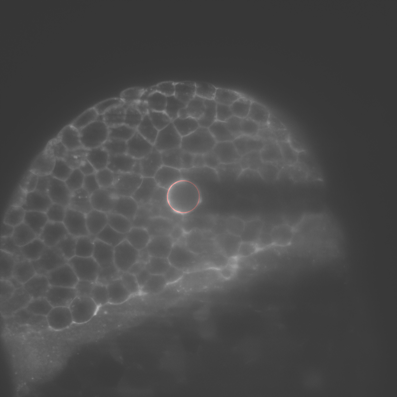
\includegraphics[width=\linewidth]{Chapters/tweezers/Figs/PDF/bead_tracked}
  \caption{Here, the red circle represents a well localised single bead.}\label{fig:bead_tracked}
 \end{subfigure}\\\vspace{\abovecaptionskip}
 \begin{subfigure}[t]{\textwidth}
  \centering
  \includegraphics{Chapters/tweezers/Figs/PDF/bead_correlation}
  \caption{
  Template matching of an ideal fluorescent bead, with a volume of \gls{zebrafish} tissue, produces a volume image with a single maximum peak where the bead resides.
  %Template matching of an ideal fluorescent bead with a volume of \gls{zebrafish} produces a volume image with a single maximum peak of where the bead resides
  }\label{fig:bead_correlation}
 \end{subfigure}%
 \caption{Template matching is used to localise bead positions through time and in 3D.
 }
\end{figure}

\subsubsection{Sub-pixel tracking}

During template matching, the output of the cross-correlation of a template and an image volume has a maximum value at the position where correlation is the highest.
For the described algorithm, the highest peak is the most likely candidate for a bead being matched.
As such, the simplest way of tracking a bead in a window is to return the cartesian coordinates of that largest value pixel.
However, the pixel values in the immediate vicinity of the highest pixel value steadily ramp up.
This phenomenon is overcome by fitting a smooth Gaussian local to the maximal peak, allowing a sub-pixel resolved series of coordinates to be found.
A more complicated, but more accurate, technique for sub-pixel tracking is to fit a b-spline to the data.
The result of a spline fitting offers a smooth fit to what is assumed to be continuous, smooth data, so that the spline itself interpolates the underlying data. Therefore, large bead positioning accuracy can reach beyond the diffraction limit.

% The output of the cross correlation of a template and an image volume will have a maxima at the position where correlation is the highest.
% For the dexcribed algorithm the highest peak is the most likely candidate for a bead being matched.
% As such, the simplest way of tracking a bead in a window requires returning the cartesian coordinates of that largest pixel.
% However, the pixel values in the immediate vicinity of the highest pixel value will steadily ramp up.
% By fitting a smooth Gaussian local to the maximal peak a sub-pixel resolved series of coordinates may be found.
% More complicated but more accurate technique for sub-pixel tracking involves the fitting of an b-spline.
% The result of a spline fitting offers a smooth fit to what is assumed continuous smooth data, the spline itself will interpolate the underlying data.
% To this end large bead positioning accuracy can reach beyond the diffraction limit.
%Not much on this..
\subsection{Cell tracking}

In addition to studying the movement of the bead, we also investigated the movement of nearby cells, with respect to the bead being moved.
To track their movements and deformation, a 3D watershed algorithm was written in IDL and applied to membrane-only imaging data.
A two-colour \gls{zebrafish} imaging technique was considered wherein one channel was fluorescent in the nuclei, whilst another channel was fluorescent exclusively in the membranes.
However, the time resolution would have had to have been halved to allow for this, given the system constraints.
Although it was possible to add a dichroic image splitter or an additional camera if necessitated, this approach would have halved the overall image resolution in the \(y\) axis, and would have added significant complexity and cost.
And so, imaging the membranes exclusively provided sufficient information to elucidate the movement and deformation of cells in close proximity to the bead.

% The actions of nearby cells with regard to the bead being moved were also of importance, to track their movements and deformation a 3D watershed algorithm written in IDL was applied to membrane-only data imaging data.
% Having a two-colour \gls{zebrafish} whereby one channel was fluorescent in the nuclei whilst another exclusively in membranes was considered.
% However, the time resolution would have needed to have been halved to allow for this given the system constraints.
% Alternatively having a dichroic image splitter or an additional camera to be added was possible.
% This approach would have halved the overall image resolution in the $y$ axis and an additional camera would have been a time-costly as well as monetarily expensive solution.

\section{Results}

%TODO Check this!
%\subsection{Ellipsoid to sphere transformation in early embryogenesis is dominated by cell motility and migration} %Lay out background of transformation
%After fertilisation, the \gls{zebrafish} embryo undergoes series of synchronous cell divisions, followed by the first morphogenetic transformations.
%Before the embryo begins its epibolic spread over the yolk cell, an initial subtle transformation occurs.
%The embryo undergoes a change in shape from an ellipsoid, at high stage (3.3hpf), to a sphere at sphere stage (4hpf) (Figure 1.A-D) (Kimmel staging).
%This involves both a reshaping of the blastula and its boundary with the yolk cell.
%To quantify this transition, an ellipse was fitted around the projected shape of the embryo and a ratio taken of the major (animal-vegetal axis, AV, R1) to the minor (equatorial, R2) diameters.
%At high stage this ratio is about 1.2 (mean = 1.18 ± 0.078 s.d.) (Figure1.E), meaning that the embryo is longer along AV axis.
%During development, this aspect ratio decreases (p1k-cell/high = 0.01534, phigh-oblong = 3.585e-05, poblong/high = 1.244e-04).
%By sphere stage, this ratio has reduced to ~1 (mean = 1.056 ± 0.053 s.d.), i.e. closer to spherical (phigh/sphere < 2.2e-16).

%These transformations are coincident with a reduction in cell volume through cell division and a concomitant reorganisation of extracellular space. (Figure S1).
%Throughout these stages, cells remain relatively loosely packed (Figure S1).
%Little is known about of the cellular or molecular basis of this transition.
%Cells acquire motility after the mid-blastula transition (Kane \& Kimmel, 1993).
%We transplanted cells expressing the actin cytoskeleton reporter Lifeact into a non-labelled recipient embryo (Figure 1.F,I), then tracked their movements and shapes in 3D.
%Cells move extensively in all three directions, with no strong orientation preference (Figure 1.G,H).
%Indeed, transplanted cells become dispersed in a manner reminiscent of diffusion, with a variation in mean squared displacement versus lag interval that gives an apparent diffusion coefficient of 14.6 µm2/min, (Fig s?).
%We use this diffusion coefficient as a convenient measure of cell movements.
%During this time, cells produce actin-enriched protrusions (Figure1.F, I).
%Surprisingly, while these protrusions show no preferred orientation within the plane parallel to the embryo surface (p = 0.606) (Figure 1.J), there is a strong orientation of protrusion along the AV axis (p = 0.0053) (Figure 1.K).
%Thus, the stereotypical tissue morphogenesis that shapes the embryo into a sphere is coincident with extensive cell mixing and polarised protrusive activity.
%Take from Julien's stuff
\subsection{Micro-rheology reveals an increase in the stiffness and elasticity of cells during high- to sphere- stage transition}

Even though it has been speculated that morphogenetic change must depend upon changes in the physical properties of tissues, there is little direct evidence to support this idea.
This study intended to verify whether the changes that are observed in cell movements and protrusive activity during the high- to sphere-stage transition, were accompanied by a modulation of physical properties of the blastoderm.
To address this question, magnetic tweezers were used to apply a direct a known force to a \SI{40}{\micro\meter} diameter superparamagnetic bead implanted into the blastoderm~\cite{fisherThreedimensionalForceMicroscope2005}. %, and push-pull experiments were performed to extract viscoelastic properties of the developing \gls{zebrafish}.
Beads were implanted in blastula-stage embryos and the cells surrounding them were imaged for up to 8 hours.
No changes were detected in local cell arrangement, actin-cytoskeleton organisation or myosin localisation around the beads.
Embryos containing a bead developed unperturbed by its presence.

% Even though it has been speculated that morphogenetic change must depend upon changes in the physical properties of tissues, there is little direct evidence to support this idea.
% We wish to ask if the changes that we see in cell movements and protrusive activity during the high- to sphere-stage transformation are accompanied by a modulation of physical properties of the blastoderm.
% To address this question, magnetic tweezers were used to apply a direct and known force to a 40 \SI{40}{\micro\metre} diameter super paramagnetic bead implanted into the blastoderm \cite{}.(%TODO reference).
% %This device creates a 3D graded magnetic field within the volume between four iron poles surrounding a suspended \gls{zebrafish} embryo.
% %The device has been calibrated to deliver known forces along three orthogonal axes (see M\&M).
% %[fluorescent beads covered with poly siloxane]

Beads were implanted in blastula-stage embryos and the cells surrounding them were imaged for up to 8 hours.
%We detected
No changes in local cell arrangement, actin cytoskeleton organisation or myosin localisation around the beads were detected.
Embryos containing a bead developed unperturbed by its presence.
The physical properties of the tissue were measured by applying a calibrated, constant force (in the order of \SI{8}{\milli\newton}) for \SI{1}{\minute} and tracking the displacement of the bead during, and after, force application.
Force was directed alternately radially towards or away from the yolk at \SI{3}{\minute} min intervals.
Bead trajectories revealed that embryonic tissue acts as a viscoelastic medium.
Trajectories invariably showed an initial fast displacement followed by a slower, linear displacement, or \emph{creep}, see \figurename~\ref{fig:combined_displacement}.
Upon release, the bead recoiled rapidly towards its original position in a reversal of the initial fast displacement.
Displacement during the slower creep phase was not recovered, see \figurename~\ref{fig:combined_displacement}.
Between high- to sphere-stage there was a significant and systematic reduction in the magnitudes of all phases of movement, but not in the overall shapes of these trajectories, see \figurename~\ref{fig:combined_displacement}.

% Beads were implanted and them and the cells surrounding them were image in blastula-stage embryos for extensive periods (up to 8 hours) and detected no changes in local cell arrangement, actin cytoskeleton organisation or myosin localisation around the beads.
% Embryos containing a bead developed unperturbed by its presence.
% %Beads were implanted and the cells surrounding them in blastula-stage embryos for extensive periods and detected no changes in local cell arrangement, actin cytoskeleton organisation (assessed with GFP-lifeact) or myosin localisation (GFP-MII). %TODO Check this in text
% %Embryos containing a bead developed, as far as we are able to detect, unperturbed by its presence.
% The physical properties of the tissue were measured by applying a calibrated, constant force (in the order of \SI{8}{\nano\metre}) for \SI{1}{\minute} and tracking the displacement of the bead during and after application.
% Force was directed alternately radially towards or away from the yolk at \SI{3}{\minute} intervals.
% Bead trajectories reveal that embryonic tissue acts as a viscoelastic medium.
% Trajectories invariably show an initial fast displacement followed by a slower, linear displacement or creep, see Figure \ref{fig:combined_displacement}.
% Upon release, the bead recoils rapidly towards its original position in a reversal of the initial fast displacement.
% Displacement during the slower creep phase is not recovered, see Figure \ref{fig:combined_displacement}.
% Between high- to sphere-stage there was a significant and systematic reduction in the magnitudes of all phases of movement but not in the overall shapes of these trajectories, see Figure \ref{fig:combined_displacement}.

To quantify and further characterise these findings, a parameterised mechanical model (Equation~\eqref{fig:combined_displacement}), that accounts for the shapes of bead trajectories over time, was fit.
The most parsimonious model consisted of a dash-pot in series with a parallel spring and dash-pot, see \figurename~\ref{fig:viscoelastic_model}.
The dash-pots are characterised by viscous coefficients, \gls{eta_1_visc} and \gls{eta_2_visc}, and the spring by an elastic modulus, \gls{E_visc}.
Fitted parameters revealed that \gls{E_visc} increased by 3 fold
(\(E_{\SI{0}{\minute}}=\SI{2.61(57)}{\pascal}\);
\(E_{\SI{75}{\minute}}=\SI{7.98(250)}{\pascal}\))
and \gls{eta_1_visc} increased 1.8 fold
(\(\eta_{1_{\SI{0}{\minute}}}=\SI{156.1(583)}{\pascal\second}\);
\(\eta_{1_{\SI{75}{\minute}}}=\SI{286.85(6934)}{\pascal\second}\))
and \gls{eta_2_visc} 2.5 fold
(\(\eta_{2_{\SI{0}{\minute}}}=\SI{15.82(320)}{\pascal\second}\);
\(\eta_{2_{\SI{75}{\minute}}}=\SI{40.20(1074)}{\pascal\second}\))
over a development time of \SI{75}{\minute}.
No significant differences were found between the two directions of force application
(\(p_E > 0.05\), \(p_{\eta_1} > 0.05\), \(p_{\eta_2} > 0.05\)).
This trend was seen irrespective of the starting developmental age of the embryo, which may suggest work hardening of the \gls{zebrafish}. %TODO Colin dont like
A characteristic time constant of the elastic deformation, \gls{tau_visc}, can be derived from the ratio of \gls{eta_2_visc} to \gls{E_visc}.
Despite large changes in both \gls{eta_2_visc} and \gls{E_visc}, \gls{tau_visc} remained largely constant over the developmental time (mean = \SI{5.33}{\second}).
This suggests that this tissue may contain a mechanism of self-regulation of \gls{tau_visc}, or that both \gls{E_visc} and \gls{eta_2_visc} are determined by a common feature.

\begin{figure}
 \centering
 \includegraphics{Chapters/tweezers/Figs/PDF/combined_displacement}
 \caption[Superraramagnetic bead movement within \gls{zebrafish} embryonic tissue]{
 Superraramagnetic bead movement within \gls{zebrafish} embryonic tissue, by a known force, shows a trajectory characteristic of viscoelastic behaviour, with a rapid elastic response (\emph{elastic phase}, comprised of the viscoelastic drive), followed by a linear creep period (\emph{creep phase}, comprised of the elastic drive). When the force is removed, the bead is recoiled (\emph{recoil phase}, comprised of a relaxation period and the end of the bead movement).
 % Paramagnetic bead moved within embryonic tissue by a known force show a trajectory characteristic of viscoelastic behaviour, with a rapid elastic response (\emph{elastic} phase), followed by a linear creep period (\emph{creep} phase).
 % When the force is removed, the bead is recoiled (\emph{recoil} phase).
 }\label{fig:combined_displacement}
\end{figure}

% %%
% To quantify and further characterise these findings, a parameterised mechanical model \eqref{eq:modelfitting} that accounts for the shapes of bead trajectories over time was fit.
% The most parsimonious model consists of a dashpot in series with parallel spring and dashpot, see Figure \ref{fig:viscoelastic_model}.
% The dashpots are characterised by viscous coefficients \(\eta_1\) and \(\eta_2\), and the spring by an elastic modulus, E.
% Fitted parameters reveal that E increased by 3 fold
% (
% \(E_{\SI{0}{\minute}}=\SI{2.61(57)}{\pascal}\);
% \(E_{\SI{75}{\minute}}=\SI{7.98(250)}{\pascal}\)
% )
% and \(\eta_1\) 1.8 fold
% (
% \(\eta_{1_{\SI{0}{\minute}}}=\SI{156.1(583)}{\pascal\second}\);
% \(\eta_{1_{\SI{75}{\minute}}}=\SI{286.85(6934)}{\pascal\second}\)
% )
% and \(\eta_2\) 2.5 fold
% (
% \(\eta_{2_{\SI{0}{\minute}}}=\SI{15.82(320)}{\pascal\second}\);
% \(\eta_{2_{\SI{75}{\minute}}}=\SI{40.20(1074)}{\pascal\second}\)
% )
% over a development time of \SI{75}{\minute}.
% No significant differences were found between the two directions of force application (\(p_E > 0.05\), \(p_{\eta_1} > 0.05\), \(p_{\eta_2} > 0.05\)).
% This trend was seen irrespective of the starting developmental age of the embryo, excluding the likelihood of work hardening as an explanation.
% %A developmental stiffening of the embryo was also seen in measurements of the apparent Young’s modulus as determined by AFM indentation (Figure S3).
% A characteristic time constant of the elastic deformation, \(\tau\), can be derived from the ratio of \(\eta_2\) to E.
% Despite large changes in both of \(\eta_2\) and E, \(\tau\) remains relatively constant over developmental time (%TODO add figure
% mean = \SI{5.33}{\second}).
% This suggests that this tissue may contain a mechanism of self-regulation of \(\tau\) or that both E and \(\eta_2\) are determined by a common feature.
%%
The proposed mechanical models provide a good explanation for the trajectory of the bead during the active force application and the initial recoil period. However, bead movements in the later recovery period were more erratic and were not accounted for by the model.
Potentially, these deviations may have resulted from additional processes, such as active cell movements.
The fitted mechanical model implies that the tissue can be described by two mechanical elements, namely, a soft viscoelastic component and a purely viscous component.
A simple hypothesis would be that the viscoelastic component derives from the mechanics of individual cells, whereas the viscosity component is a measure of cell-cell interaction.
This was addressed in two ways.
Firstly, changes in cell shapes and rearrangements within the tissue, both during and after bead movement, were visualised and measured;
secondly, these measurements were repeated in embryos in which there had been a manipulation of cell adhesion, cell protrusive activity and cell contractility, thereby testing the roles of these parameters in determining mechanical properties.

% %%
% The proposed mechanical models provides a good explanation for the trajectory of the bead during the active force application and the initial recoil period.
% However, bead movements in the later recovery period are more erratic and not accounted for by the model.
% Potentially, these deviations may result from additional processes, such as active cell movements.
%
% %GOOD /\
% The fitted mechanical model implies that the tissue can be described by two mechanical elements, a soft viscoelastic component and a pure viscous component.
% %We now asked if these mechanical descriptors can be understood in terms of cellular characteristics of the tissue.
% A simple hypothesis would be that the viscoelastic component derives from the mechanics of individual cells, and the purely viscosity component is a measure of cell-cell interaction.
% This was addressed in two ways.
% Firstly, changes in cell shapes and rearrangements within the tissue during and after bead movement were visualised and measured; secondly, these measurements were repeated in embryos in which there had been a manipulation of cell adhesion, cell protrusive activity and cell contractility testing their roles in determining mechanical properties.

%%
%\begin{figure}
% \centering
% \hfill
% \begin{subfigure}[t]{1\linewidth}
%  \centering
%  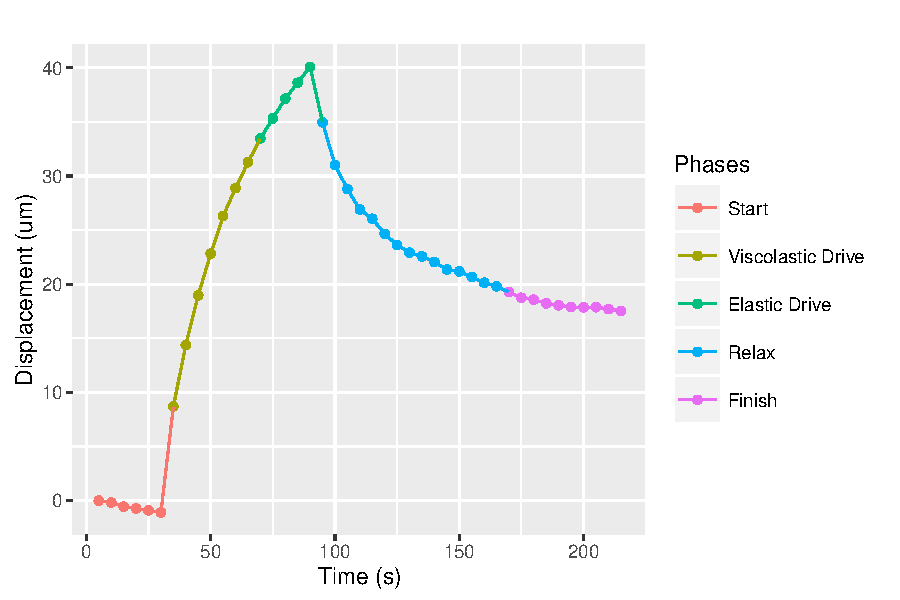
\includegraphics{Chapters/tweezers/Figs/PDF/Displacement_Plot}
%  \caption{Unfiltered reconstruction using a radon transform}
%  \label{fig:}
% \end{subfigure}\hfill
% \begin{subfigure}[t]{1\linewidth}
%  \centering
%  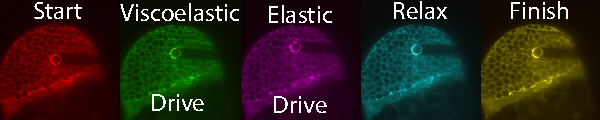
\includegraphics{Chapters/tweezers/Figs/PDF/coloured_fish_stages}
%  \caption{Snapshots in time of each of the stages of drive and recovery.}
%  \label{fig:filtered_recon_helix}
% \end{subfigure}
%  \hfill
%  \label{fig:flopts}
% \caption{Comparison of the two reconstructions under sample imaging with a systematic drift, in 3D though represented here in 2D.}
 %\end{figure}

 \begin{figure}
 \centering
 \hfill
  \begin{subfigure}[t]{1\linewidth}
   \centering
   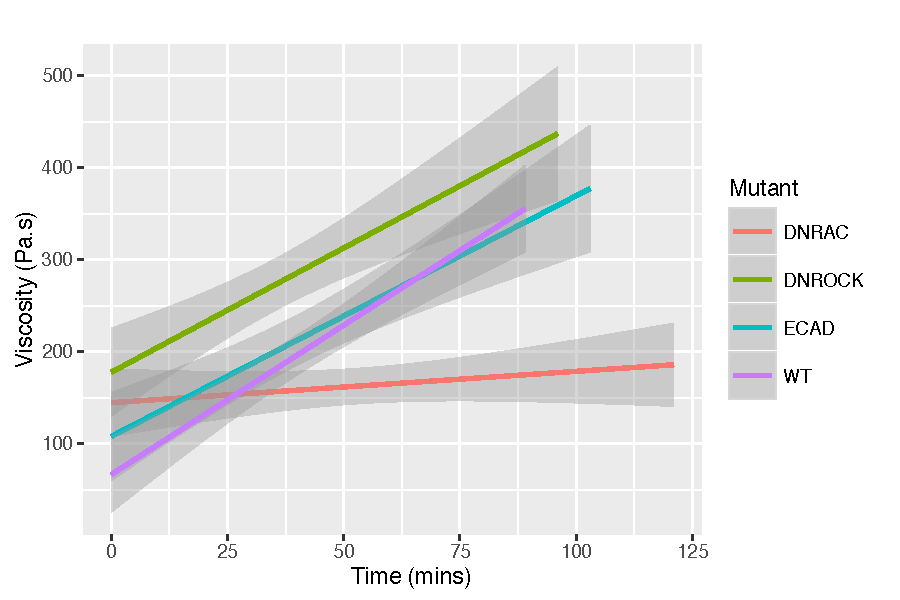
\includegraphics{Chapters/tweezers/Figs/PDF/Cells_-_Time}
   \caption{Change of cellular viscosity \gls{eta_1_visc}, over time}\label{fig:cells_time}
  \end{subfigure}\hfill
   \begin{subfigure}[t]{1\linewidth}
    \centering
    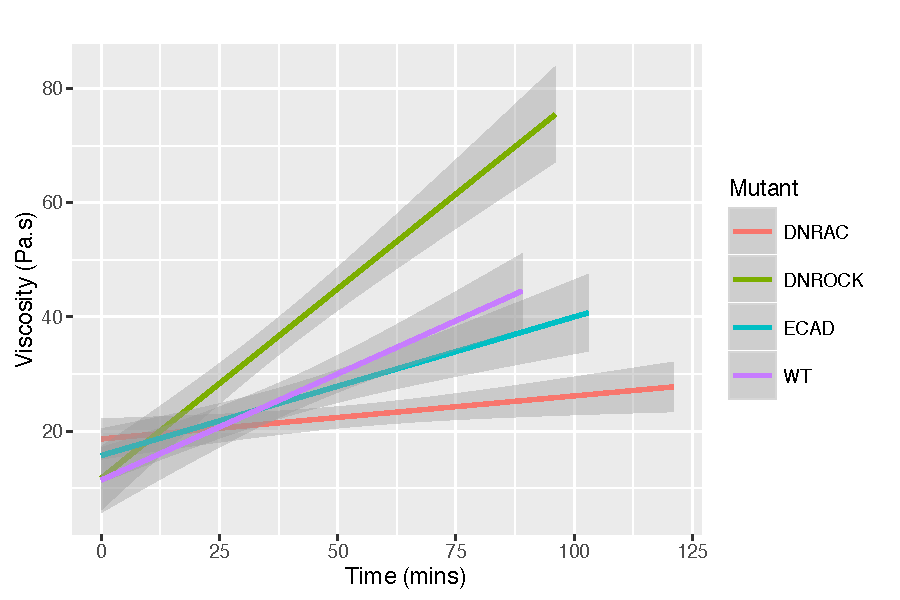
\includegraphics{Chapters/tweezers/Figs/PDF/Tissue_-_Time}
    \caption{Change of tissue viscosity \gls{eta_2_visc} over time}\label{fig:tissue_time}
   \end{subfigure}\hfill
\end{figure}
\begin{figure}
  \ContinuedFloat{}
   \begin{subfigure}[t]{1\linewidth}
   \centering
   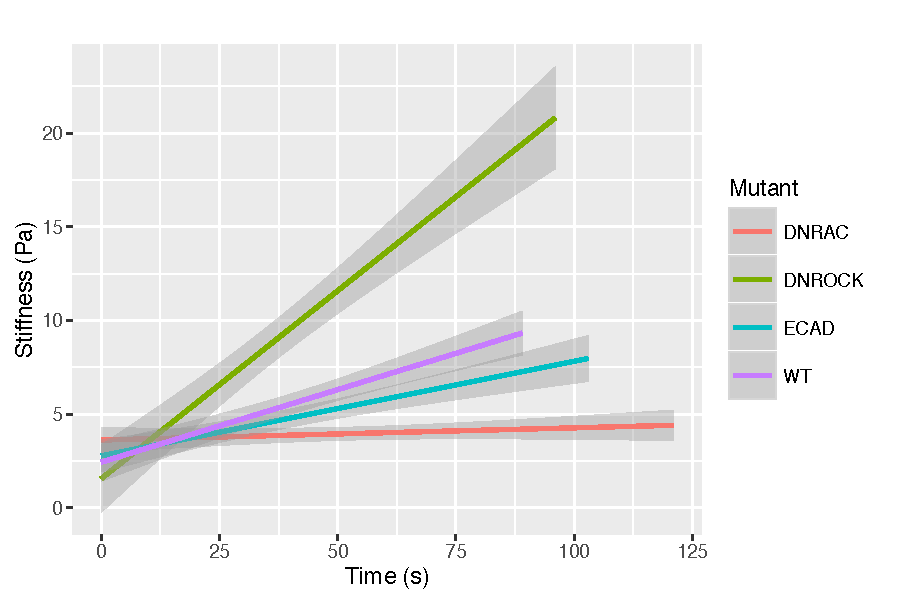
\includegraphics{Chapters/tweezers/Figs/PDF/Stiffness_-_Time}
   \caption{Change of elastic modulus \gls{E_visc}, over time}\label{fig:stiffness_time}
  \end{subfigure}\hfill
  \caption[Genetic knockdowns have consequences on the developmental evolution of rheological parameters in \gls{zebrafish}]{
Genetic knockdowns have consequences on the developmental evolution of rheological parameters in \gls{zebrafish}, viscosity coefficients, \gls{eta_1_visc} (a\ref{fig:cells_time}) and \gls{eta_2_visc} (\subref{fig:cells_time}), and elastic modulus, \gls{E_visc} (\ref{fig:stiffness_time}), are decreased in MoECad (n=151 pulls, 9 embryos), and \gls{DNRAC} (n=158 pulls, 9 embryos) genotypes, while they are increased in the \gls{DNROCK} (n=107 pulls, 9 embryos) genotype compared to \gls{WT} (n=178 pulls, 9 embryos).
Not experiments are shown to terminate together as some specimens did not survive the full \SI{2}{\hour} course of the experiment.
 %
 % These knock downs have consequences on the developmental evolution of rheological parameters, viscosity coefficients \gls{eta_1_visc} \ref{fig:cells_time} and \gls{eta_2_visc} (\ref{fig:tissue_time}), and, elastic modulus \gls{E_visc} (\ref{fig:stiffness_time}):
 % they are decreased in MoECad (n=151 pulls, 9 embryos), and \gls{DNRAC} (n=158 pulls, 9 embryos) while they are increased in \gls{DNROCK} (n=107 pulls, 9 embryos) compared to \gls{WT} (n=178 pulls, 9 embryos).
  }\label{fig:visco_time}
\end{figure}

\subsection{Elasticity is linked with cell shape deformation and viscosity with cell rearrangement}

To examine how cells around the bead responded during the force application fast volumetric light-sheet imaging combined with magnetic tweezers enabled the simultaneous tracking of cell shapes and positions during mechanical probing (\figurename~\ref{fig:cell_tracking}a-b).
The time course was partitioned into five epochs, based upon the experimental protocol, and the mechanical signatures as described above.
The elastic phase was defined as \(3\times\gls{tau_visc}\) (spanning \SI{95}{\percent} of the elastic duration).
The remaining period of active bead displacement was defined as the creep phase.
Finally, a 3\gls{tau_visc} period of elastic recoil was analysed as the recoil period.
Cell outlines and positions were automatically tracked, manually omitted and corrected.
Cell shape changes and cell displacements were measured along the axis of force application to the bead.

% To examine how cells around the bead responded during the force application, fast volumetric light-sheet imaging combiend with magnetic tweezers enabled the simultaneously tracking of cell shapes and positions during mechanical probing (Figure \ref{fig:cell_tracking} A-B).
% The time course was partitioned into five epochs, based upon the experimental protocol and the mechanical signatures as described above.
% %We look for cellular correlates of bead displacement in the phases labelled elastic, creep and recoil.
% The elastic phase is defined as \(3\times\gls{tau_visc}\) %where $\tau$ is the viscoelastic time constant
% (spanning \SI{95}{\percent} of the elastic duration).
% The remaining period of active bead displacement is defined as the creep phase.
% Thirdly, a $3\tau$ period of elastic recoil was analysed as the recoil period.
% Cell outlines and positions were automatically tracked and manually omitted and corrected.
% Cell shape changes and cell displacements are measured along the axis of force application to the bead.

Four sectors were defined around the bead relative to this axis (\figurename~\ref{fig:cell_tracking}a); here, only the front and rear sectors were considered.
In front of the bead, during the elastic period, cells were both compressed and displaced forward by its movement (\figurename~\ref{fig:cell_tracking}c-d).
This tendency of cells to deform diminished over development time (\figurename~\ref{fig:cell_tracking}f, \(p_\text{linear-regression} = 0.016\)). %ROX r^2
In fact, cell shape strain rates were highly correlated with, and largely account for, tissue deformation strain rate (\figurename~\ref{fig:cell_tracking}f,	\(p\text{correlation} = 0.0001757\), \(R^2 = 0.743\)).
The cell shape strain rate coefficient correlated with \gls{E_visc} (\figurename~\ref{fig:cell_tracking}i, \(p_\text{correlation} = 0.0449\), \(R^2 = 0.453\)).
Behind the bead, we observed a complementary pattern of cell and tissue stretching (\(p_\text{correlation} = 0.0748\), \(R^2 = 0.473\)) at all except the earliest developmental stages.
Incomplete cell adhesions, which in turn created holes in the tissue when the bead moved with excess force, may be the cause of this effect.
For these cases, cell shape change strain rates did not correlate with tissue deformation strain rate.
When the magnetic force was no longer applied, previously compressed cells ahead of the bead re-expanded back along the force axis (\figurename~\ref{fig:cell_tracking}d, h \(p_\text{linear-regression} = 0.016\)). %ROX r^2
Previously stretched cells behind the bead then contracted as the bead recoiled backwards (\figurename~\ref{fig:cell_tracking}d).
There was a strong correlation between \gls{E_visc} and the rate of expansive cell shape deformation in front of the bead (\figurename~\ref{fig:cell_tracking}k, \(p_\text{correlation} = 0.016\), \(R^2 = 0.53\)).
This is consistent with the rapid elastic bead recoil being determined by an elastic recoil in cell shape, after the release of the imposed force.
In conclusion, the cellular signature of the elastic periods were largely accounted for by cell shape deformations.

% Four sectors were defined around the bead relative to this axis (Figure \ref{fig:cell_tracking} A); here only the front and rear sectors are considered
% %As a first approximation, to assess how tissue is elastically-deformed in space, we use an elastic medium force point formula (ref) that couples cell dissplacement inversely to distance from the centre of force application (the bead), and for a cell shape change stain rate, we use the derivative of this formula.
% In front of the bead, during the elastic period, cells are both compressed and displaced forward by its movement (Figure \ref{fig:cell_tracking} C,D).
% This tendency of cells to deform diminishes over development time (Figure \ref{fig:cell_tracking} F, $p_\text{linear-regression} = 0.016$).
% In fact, cell shape strain rates are highly correlated with and largely accounts for tissue deformation strain rate (Figure \ref{fig:cell_tracking} F, $p_\text{correlation} = 0.0001757$, $R^2 = 0.743$).
% Cell shape strain rate coefficient is correlated with E (Figure \ref{fig:cell_tracking} I, ${p_\text{correlation}} = 0.0449$, $R^2 = -0.453$).
% Behind the bead, we can see a complementary pattern of cell and tissue stretching ($R^2 = 0.473$, $p = 0.0748$), at all except the earliest developmental stages.
% Incomplete cell adhesions which in turn create holes in the tissue when the bead movies with excess force, may be the cause of this effect.
% %This may be due to incomplete cell adhesion, creating holes in the tissue when the bead moves with excess force.
% For these cases, cell shape change strain rates are not correlated with tissue deformation strain rate.
% When the magnetic force is no longer applied, previously compressed cells ahead of the bead re-expand back along the force axis (Figure $p_\text{linear-regression} = 0.016$) D,H).
% Previously stretched cells behind the bead would then contract as the bead recoiled backwards (Figure \ref{fig:cell_tracking} D).
% There is a strong correlation between E and the rate of expansive cell shape deformation in front of the bead (Figure \ref{fig:cell_tracking} K, $R^2 = 0.53$, $p = 0.016$).
% This is consistent with the rapid elastic bead recoil being determined by an elastic recoil in cell shape, after the release of the imposed force.
% In conclusion the cellular signature of the elastic periods are largely accounted for by cell shape deformations.

% \begin{landscape}
 \begin{figure}
 \centering
  \includegraphics[width=\linewidth]{Chapters/tweezers/Figs/PDF/cell_tracking_2} %TODO In addition to Colin’s comments here, make sure the axis labels are centred, and correct spelling in y axis of panel I
  % \caption{p.t.o}
%  \end{figure}
% % \end{landscape}
% \begin{figure}\ContinuedFloat
 \caption[Sketch of the dynamics in a typical rheological experiment]{\footnotemark{}
 Sketch of the dynamics in a typical rheological experiment (a) in \gls{WT} embryo under \gls{LSFM} (b), where blue represents cell extension and red represents compression.
 In (a) the labels 1, 2 and 3 follow respective cells over time.
 The yellow dot in the \gls{LSFM} images marks the original position  of the bead centre.
 (c)~-~(d): Analysis of the coefficient of deformations \(C_t\) and \(C_C\) showed that tissue (c) and cells (d) were compressed at the front  of the bead while they were stretched at the rear during bead  pulling (n = 14 pulls, 3 embryos).
 (e)~-~(h): Analysis of cell area  and cell aspect ratio revealed that cells disappear from the imaging plane, suggesting that cells at the front rearranged in 3D, while at the rear, cells were stretched (e).
 Along developmental time, tissue deformation (\(C_t\)), cell deformation \(C_C\) and cell intercalation (\(C_t\)-\(C_s\) during elastic phase (in \SI{}{\micro\metre\squared\per\minute})), at the front of the bead, show that tissue compression could be accounted for mainly by cell shape changes (f), while, during creep phase, strain rates showed that this accountancy is lost, suggesting cell rearrangement is a major event (g).
 When the force was released, cells at the front relaxed to their original shape (h).
%  p.t.o.}
% \end{figure}
% \begin{figure}
%   \ContinuedFloat{}
%   \caption{
(i)~-~(k): Correlation analysis of cell parameters and rheological parameters.
This is supported by correlations between elastic modulus, \gls{E_visc}, and cell shape change coefficient during elastic phase, at the front of the bead (i), between viscosity coefficient, \gls{eta_1_visc}, and cell rearrangement rate during creep phase (j), and between elastic modulus, \gls{E_visc}, and cell shape change coefficient during recoil phase (k).
Lines represent linear regressions.
% A-B: Sketch of typical rheological experiment (A) in \gls{WT} embryo under SPIM (B) where blue represents cell extension and red is compression. 1-2-3 label regarding cells over time-lapse.
% Yellow dot marks the original position of the bead centre.
% C-D: Analysis of the coefficient of deformations \(C_t\) and \(C_C\) shows that tissue (C) and cells (D) are compressed at the front of the bead while they are stretched are the rear during bead pulling (n = 14 pulls, 3 embryos).
% E-H: Analysis of cell area and cell aspect ratio reveals cells disappear from imaging plane, suggesting cells at the front rearrange in 3D, while at rear, cells are stretched (E).
% Along developmental time, tissue deformation (\(C_t\)), cells deformation (\(C_c\)) and cell intercalation (\(C_t\)-\(C_s\)) during elastic phase (in \SI{}{\micro\metre\squared\per\minute}), at the front of the bead, show that tissue compression can be accounted mainly by cell shape changes (F), while, during creep phase, strain rates show that this accountancy is lost, suggesting cell rearrangement is major event (G).
% When force is released, cells at the front relax to their original shape (H).
% I-K: Correlation analysis of cell parameters and rheological parameters.
% This is supported by correlations between elastic modulus E and cell shape change coefficient during elastic phase, at the front of the bead (I), between viscosity coefficient \gls{eta_1_visc} and cell rearrangement rate during creep phase (J), between elastic modulus \gls{E_visc} and cell shape change coefficient during recoil phase (K).
% Lines represent linear regressions.
}\label{fig:cell_tracking}
\end{figure}
\footnotetext{Figure currently being prepared for publication, reproduced with permission from Dr.~Julien Dumortier}
To investigate how tissue deforms during the creep phase, which is defined by \gls{eta_1_visc} in the mechanical model, the behaviour of cells in the tissue at the front and rear of the bead were visually inspected.
Cells became more compressed and moved out of the imaging plane (decreasing in area) in front of the bead and, conversely, cells became stretched and entered  the plane at the rear (\figurename~\ref{fig:cell_tracking}a-b).
This behaviour may be quantified by comparing changes in cell aspect ratio and area through both the elastic and creep periods (\figurename~\ref{fig:cell_tracking}e).
Early cell shape changes gave way to area changes during the creep period; this may be interpreted as the result of cells rearranging in the tissue in front of and behind the bead.

% To investigate how tissue deforms during the creep phase, which in the mechanical model is defined by $\eta_1$, the behaviour of cells in the tissue at the front and rear of the bead were visually inspected.
% Cells became more compressed and would moved out the plane (decreasing in area), in front of the bead and conversely cells would become stretched and enter the plane at the rear (Figure \ref{fig:cell_tracking} A, B).
% This behaviour may be quantified by comparing changes in cell aspect ratio and area through both the elastic and creep periods (Figure \ref{fig:cell_tracking} E).
% Early cell shape changes give way to area changes during the creep period, this may be interpreted as the result of cells rearranging in the tissue in front and bead the bead.
%%%%

While the elastic periods were dominated by changes in cell shape, the creep period was characterised by cell rearrangements.
Cell shape strain accounted for a small fraction of tissue strain rate (\figurename~\ref{fig:cell_tracking}g), and did not correlate with \gls{eta_1_visc}
(\(R_\text{front}^2 = 0.345\), \(p = 0.21\); \(R^2 =	0.052\), \(p = 0.85\)).
Nonetheless, measurable cell shape strain rates indicated that some contribution persisted through the creep period.
However, cell intercalation strain rate correlated with \gls{eta_1_visc}, both in front of (\figurename~\ref{fig:cell_tracking}j)
(\(p_\text{correlation} = 0.0638\), \(R^2 = 0.49\)) and behind the bead (\(p = 0.035\), \(R^2 =	0.546\)).
Cell rearrangements appeared to be the major determinants of tissue viscosity in the creep period.

% %To quantify cell behaviours during the creep period, we measure cell and tissue strain rates using a simplified tissue tectonics approach (REF).
% %Tissue strain rate, cell shape strain rate and cell rearrangement rates are measured along the direction of force application (see M\&M).
% While the elastic periods were dominated by changes in cell shape, the creep period is characterised by cell rearrangements.
% Cell shape strain accounts for a small fraction of tissue strain rate (Figure \ref{fig:cell_tracking} G), and does not correlate with $\eta_1$ ($R_\text{front}^2 = 0.345$, $p = 0.21$; ($R_\text{rear}^2 = -0.052$, $p = 0.85$).
% Nonetheless, measurable cell shape strain rates indicate that some contribution persists through the creep period.
% However, cell intercalation strain rate does correlate with $\eta_1$, both in front (Figure \ref{fig:cell_tracking} J) $p_\text{correlation} = 0.0638$, $R^2 = 0.49$) and behind the bead ($p = 0.035$, correlation $= -0.546$).
% Cell rearrangements appear to be the major determinants of tissue viscosity in the creep period.

%Good \/
%
\subsection{Modifications of cell motility and migration lead to defects in early embryogenesis and tissue rheology}

The results of analysing movement during bead displacement were consistent with our simple hypothesis of a two-component model in which the viscoelastic component of tissue perturbation is derived from the mechanics of individual cells, while the component designating only viscosity is a measure of cell-cell interaction.
To study how changes in these parameters affect embryo development, and the mechanical properties of the blastoderm, we employed a genetically altered line of zebrafish deficient in E-Cadherin (CDH1) expression.
E-Cadherin is an essential transmembrane protein which mediates cellular adhesion, a fundamental requirement for building a cohesive tissue.
To achieve this, we employed a knockdown Morpholino approach (MoECad)~\cite{babbEcadherinRegulatesCell2004} for cell adhesion, which lead to defects in the high-to-sphere transformation;
these embryos failed to achieve a spherical shape (\figurename~\ref{fig:cell_tracking}a).
Rheological measurements showed that MoECad-treated embryos remained less stiff and less viscous than their wildtype counterparts.
Furthermore, they were reduced in their ability to elevate these properties over developmental time (\figurename~\ref{fig:visco_time}), resulting in developmental trends that were significantly different to the \gls{WT} genotype.
Cell migration and cell protrusive activity are two important cell behaviours in the blastoderm.
Small enzymes able to hydrolyse the nucleotide guanosine triphosphate (termed GTPase enzymes) have been identified as central orchestrators of cell polarity and motility~\cite{machacekCoordinationRhoGTPase2009}.
Thus, we manipulated two complementary GTPase components of cell protrusion and migration.
The signalling of the GTPase \gls{Rac1} was inactivated by using a \gls{DNRAC}~\cite{tahinciDistinctFunctionsRho2003}.
The same approach was employed to inactivate the signalling of the GTPase \gls{RhoA} by introducing a \gls{DNROCK}~\cite{witzelWnt11ControlsCell2006}.
\gls{DNRAC} has been shown to eliminate protrusive activity mediated by \gls{Rac1}~\cite{tahinciDistinctFunctionsRho2003}, while \gls{DNROCK} has been shown to reduce the activation of the molecular motor, myosin II, which mediates cellular migration~\cite{vicente-manzanaresNonmuscleMyosinII2009,
vicente-manzanaresRegulationProtrusionAdhesion2007}. %ROX Need references for DNRAC function, DNROCK function, and the fact that  myosin II is involved in cellular migration (recommend vincente-manzanares 2009, nat rev mol cell boil.)
The injection of these dominant negative constructs affected early morphogenesis; \gls{DNRAC}-injected embryos failed to progress to a spherical shape, while \gls{DNROCK} injection caused an accelerated high-to-sphere transition.
As expected, our measurement of these rheological parameters by magnetic bead displacement confirmed these predictions: \gls{DNRAC} embryos failed to increase in stiffness and viscosities \gls{eta_1_visc} and \gls{eta_2_visc}
(\( p_{\gls{E_visc}} = \SI{1.016e9}{} \),
\( p_{\gls{eta_1_visc}} = \SI{1.876e4}{} \),
\( p_{\gls{eta_2_visc}} = \SI{0.0028}{} \)), while \gls{DNROCK} embryos became stiffer and more viscous
(\(p_E = 7.59e-25\),
\(p_{\gls{eta_1_visc}} = \SI{6.74e-15}{}\),
\(p_{\gls{eta_2_visc}} = \SI{3.65e-12}{}\)) than their \gls{WT} counterparts (\figurename~\ref{fig:cell_tracking}f~-~\ref{fig:cell_tracking}h) \gls{tau_visc} was affected by these knockdowns, as stiffer embryo showed a shorter \gls{tau_visc} than softer ones (\(p \ll 1e-5\)).

\subsection[Changes in rheological properties for DNRAC and DNROCK treatments are reflected in the rates of cell and tissue deformation]{Changes in rheological properties for \gls{DNRAC} and\\ \gls{DNROCK} treatments are reflected in the rates of cell\\ and tissue deformation}

Fast \gls{light-sheet} imaging analyses were repeated with each knockdown treatment to follow cell behaviours during force application.
The resultant parameters segregated according to their mechanical properties: softer \gls{DNRAC} embryos presented more cell deformation during the elastic period (\(p_\text{\gls{WT}-\gls{DNRAC}} = 0.0013\)) and more cell rearrangement during the creep period (\(p\text{\gls{WT}-\gls{DNRAC}} = 0.0025\)), compared to \gls{WT}.
Cells in the stiffer \gls{DNROCK}-injected embryos deformed less in the elastic period (\(p\text{\gls{WT}-\gls{DNROCK}} = 0.0017\)) and exhibited fewer cell rearrangements in the creep period (\(p\text{\gls{WT}-\gls{DNROCK}} = 0.0013\)) (\figurename~\ref{fig:cell_tracking}j).
These results confirm that the previously-observed correlations between cellular and rheological parameters hold true under this expanded range;
stiffness, \gls{E_visc}, is strongly correlated with initial cell shape deformation, while \gls{eta_1_visc} is strongly correlated with cell rearrangements.
This suggests that there may be a relatively simple cellular interpretation of the physical model measured using magnetic bead rheology.

% The results of analysing %cell shape changes and
% movement during bead displacement are consistent with our simple hypothesis of a two-component model.
% %To test this hypothesis further, we have manipulated embryos to modulate their cellular properties.
% These changes affect embryo development, %cell behaviours
% and the mechanical properties of the blastoderm.
% Cell adhesion is a fundamental requirement for building a cohesive tissue, expression of E-Cadherin (cdh1) was reduced.
% Using a knock-down Morpholino approach (MoECad) for cell adhesion leads to embryos defective in the high-to-sphere transformation; these embryos failed to achieve a spherical shape (Figure \ref{fig:cell_tracking} A).
% %At a cellular level, cell protrusions lose their radial polarity (Figure S5), while the number of protrusion per cell are not different (Figure \ref{cell_tracking}B, C).
% %Further, cells in treated embryos have a reduced coefficient of diffusion (6.3 µm2/min, pWT-MoECad = 1.6*10-5), showing them less able to migrate as extensively as WT cells (Figure \ref{cell_tracking}.B, p = 1.621e-05), though the directions of migration are as seen in WT ****[Check those directions].
% Rheological measurements show that MoECad-treated embryos remain less stiff and less viscous than their wildtype counterparts.
% Further, they are reduced in the elevation of these properties over developmental time \ref{fig:visco_time}
% Developmental trends are significantly different to WT, $p_E =$ \SI{5.63e-07} , $p_{\eta_1} =$ \SI{2.10e-03}, $p_{\eta_2} =$ \SI{0.042}).
%
% Cell migration and cell protrusive activity are two major cell behaviours at these stages.
% Small GTPases are identified as central orchestrators of cell polarity and motility \cite{}%TOOD cite 23.
% Two complementary molecular components of cell migration, Rac1 signalling were manipulated,
% Rac1 signalling using a dominant-negative Rac1 construct (DNRAC, \cite{}), RhoA signalling by a dominant-negative Rho-kinase construct (DNROCK, \cite{}%TOOD cite 24
% ).
% Speculatively, DNRAC should eliminate protrusive activity, while DNROCK would reduce the activation of the molecular motor myosin-2.
% The injection of these dominant negative constructs affects early morphogenesis, DNRAC-injected embryos fail to progress to a spherical shape, while DNROCK injection causes a faster round-up of the embryo.
% %Myosin-2 inhibition via blebbistatin treatment gives the same phenotype as DNROCK treatment (Figure S5).
% %At a cellular level, cells in DNRAC-injected embryos produce far fewer protrusions (Figure \ref{cell_tracking}B, freqWT = 2.05 extensions/frame/cell, freqDNRAC = 0.4 extension/frame/cell, p = 0.01386).
% %Cells in DNROCK-injected embryos make significantly more protrusions than WT (Figure \ref{cell_tracking}B, freqDNROCK = 5.30 extensions/frame/cell, p = 0.0007866) and more cells display a multipolarity (Figure \ref{cell_tracking}.C).
% %Cell protrusions in DNROCK-injected embryos favour a radial distribution but are more dispersed and numerous than WT (Figure S6).
% %The increase in protrusion production in DNROCK embryos is as expected for a loss of function of myosin-2 in migratory cells [ref].
% %(Protrusions on DNRAC injected cells are too infrequent to perform statistical analyses.)
% %Within DNRAC-injected embryos, the apparent diffusion of cells is significantly reduced compared with WT (4.3 µm2/min, pWT-DNRAC = 10-8).
% %Apparent cell diffusion in DNROCK-injected embryos is significantly increased compared with WT (29.9 µm2/min, pWT-DNROCK = 0.000433).
% %**** Analyses of cell migration directions in DNRAC are …., and in DNROCK appears as in WT (Figure S6).
% %In addition, recruitment of myosin-2 to the cell cortex is greatly reduced in DNROCK-treated cells (Figure S7).
% %Cortical myosin2 resembles the WT distribution in both DNRAC and MoECad injected embryos (Figure S7).
% %Interestingly, at both cellular and embryonic levels, the phenotypes of DNRAC and DNROCK treated embryos differ from WT in opposite ways, including embryo morphology, cell protrusion formation, cell migration and cell dispersion.
% %In the light of the MoECad results, we would predict that the physical properties of DNRAC-injected embryos should be less stiff and less viscous than WT those for DNROCK-injected would be stiffer and more viscous.
% When we measure those rheological parameters by magnetic bead displacement, we confirm these predictions: DNRAC embryos fail to increase stiffness and viscosities $\eta_1$ and $\eta_2$ ($p_E = $ \SI{1.016e-09}, $p_{\eta_1}$ = \SI{1.876e-04}, $p_{\eta_2}$ = \SI{0.0028}) while DNROCK embryos become stiffer and more viscous ($p_E =$ \SI{7.59e-25}, $p_{\eta_1}$ = \SI{6.74e-15}, $p_{\eta_2} =$ \SI{3.65e-12}) than their WT counterparts (Figure .F-H).
% Interestingly, $\tau$ is affected by the different knock downs, stiffer embryo showing a shorter $\tau$ than softer ones ($p \ll $ \SI{1e-5}).

% %TODO edit \/
% \subsubsection{How do the changes rheological properties found for DNRAC and DNROCK treatments are reflected in the rates of cell and tissue deformation?}
%
% Fast light sheet imaging analyses were repeated with each knock-down treatment, to follow cell behaviours during force application.
% The resultant parameters do segregate according to their mechanical properties: softer DNRAC embryos present more cell deformation during the elastic period ($p_\text{WT-DNRAC} = 0.0013$) and more cell rearrangement during the creep period ($p_\text{WT-DNRAC} = 0.0025$), compared to WT.
% Cells in the stiffer DNROCK-injected embryos deform less in the elastic period ($p_\text{WT-DNROCK} = 0.0017$) and induce fewer cell rearrangements in the creep period ($p_\text{WT-DNROCK} = 0.0013$) (Figure \ref{fig:cell_tracking} J).
% %We can now combine data from all WT and experimental manipulation conditions to examine correlations within an extended range of developmental conditions.
% These results confirm that the previously-observed correlations between cellular and rheological parameters hold true under this expanded range.
% Stiffness E is strongly correlated with initial cell shape deformation while $\eta_1$ is strongly correlated with cell rearrangements.
% This suggests that there may be a relatively simple cellular interpretation of the physical model measured using magnetic bead rheology.
% %As the measurement of bead movements are faster, easier and more sensitive than the associated cell measurements, this facilitate us gaining greater insight into the mechanics of developing tissues.

\begin{figure}
 \centering
 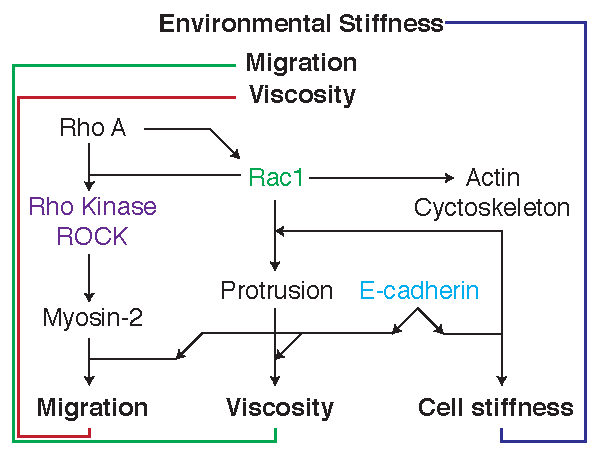
\includegraphics{Chapters/tweezers/Figs/PDF/interconnected_protein_signalling}
 \caption[Summary of effects of knockdowns in cell motion, cell protrusive activity and cell adhesion through the loss of function of \gls{Rac1}, \gls{DNROCK} and E-Cadherin]{
 Summary of effects of knockdowns in cell motion, cell protrusive activity and cell adhesion through the loss of function of \gls{Rac1}, \gls{DNROCK} and E-Cadherin.
 Based on literature, a feedback mechanism via mechano-sensing through \gls{Rac1} (blue, red and green arrows) is speculated to regulate the tissue rheology.
 \gls{Rac1} activation promotes actin cytoskeleton elaboration, increasing cell stiffness, and the production of cell protrusions.
 Protrusions provide a means of elaborating cell-cell adhesion, increasing tissue viscosity and enabling motility.
 Motility is achieved by contraction relative to points of adhesion, providing both movement and effectively testing the mechanical compliance of the cell network, feeding back to activate \gls{Rac1}.
 }\label{fig:interconnected_protein_signalling}
\end{figure}

%DONE til
\section{Discussion}

The study presented here is the first demonstration of a direct link between cell behaviours and embryo morphogenesis arising from changing mechanical properties.
By applying a directed local force to a developing embryo, through an embedded magnetic bead, local and ensemble mechanical properties of tissue were characterised.
The blastula tissue was shown to have an intrinsic viscoelastic response;
the data showed that tissues exhibit fluid-like behaviours, as observed in previous studies using optical tweezers in mature epithelia,~\cite{bambardekarDirectLaserManipulation2015} and magnetic droplets injected into much older fish than considered here~\cite{serwaneVivoQuantificationSpatially2017}.
The viscoelastic timescale parameter, \gls{tau_visc}, remained constant across both time and embryonic mutations.
The results of this study elucidate the biological meaning of the rheological parameters of viscosity and elasticity in terms of cellular morphology changes and rearrangement.

The viscous and elastic components are involved in cell shape, intercalation and deformation.
Increased stiffness is related to less deformable cells, and increased viscosity to diffusivity of cells during rearrangement.
In developing wild type embryos, prior to bulging, the blastula becomes 3-fold more viscous and stiff.
Tissue viscosity, in the form of cell rearrangement, is a measure of the friction imposed by cell-cell connections, which may be mediated by cell protrusions and
E-cadherin adhesion.
\gls{Rac1} activity would then follow to promote viscosity and cell stiffness by increasing the polymerisation of actin and encouraging cell-cell adhesions via E-cadherin connections.
Yet, the decrease in cell stiffness with MoECad treatment suggests a more complicated coupling. %ROX [of what and what? Ecad and Rac1?]
We propose that a cellular mechanotransduction mechanism assays the compliance of the environment between sites of adhesion.
It is well understood that cells grown on a surface adjust their mechanical stiffness in proportion to substrate stiffness. %ROX  [? ? ]
In the case of early mesenchymal tissues, we suggest that the cells themselves collectively constitute their own local mechanical environment, coupled via protrusion-promoted cell-cell adhesion.
Numerous examples exist of mesenchymal cells interacting via protrusions.
During collective migration, cadherin-mediated cell-cell connections are able to promote cell polarisation and cytoskeletal rearrangements, acting through \gls{Rac1} activation~\cite{caiMechanicalFeedbackEcadherin2014}.
Given the role of protrusions in both motility and transduction, this relationship explains the close correlation between viscosity and stiffness.

The emergence of cohesive mesenchymal tissue mechanical properties may be linked with the motility of its cells and, in particular, the formation of protrusions that facilitate the establishment of cadherin-based cell-cell adhesions.
Connectivity could result in an actin superstructure networked between cells, through cell adhesion proteins.
Tissue stiffness and viscosity are well-correlated with the number of protrusions present and it is possible that these mechanisms might be found in other mesenchymal tissues during development~\cite{shawkyTissueMechanicsAdhesion2015}.
These findings highlight a potentially fundamental difference in the determination of mechanical properties between epithelial and mesenchymal tissues.
Epithelial cells represent relatively static configurations, based upon adhesion and contraction, while mesenchymal cells are adhesive and stiff, but dependent upon dynamic protrusion-based motility.
The stiffening blastula, composed of radially anisotropic cells, is thus poised to drive blastula thinning and yolk bulging in the next morphogenetic movement of the zebrafish embryo.

% The study presented here has demonstrated that, for the first time, a direct link between cell behaviours and embryo morphogenesis arising from changing mechanical properties.
% By applying a directed local force to a developing embryo through an embedded magnetic bead, local and ensemble mechanical properties of tissue were characterised.
% Working in the blastula, it was shown to have an intrinsic viscoelastic response; the data compounds that tissues exhibit fluid-like behaviours with similar studies using optical tweezers in mature epithelia, \cite{19} and the use of magnetic droplets injected into much older fish than considered here \cite{18}.
% The viscoelastic time scale remained as a constant across both time and embryonic mutations.
% The results of this study provide elucidate the meaning of the rheological parameters.
% The viscous and elastic aspects are involved in cell shape and cell intercalation of the deformation.
% Larger stiffness is related with less deformable cells, and larger viscosity with diffusely of cells rearrangement.
% In developing wild-type embryos and prior to bulging the blastula becomes 3 fold more viscous and stiff.
%
% Tissue viscosity in the form of cell rearrangement, is a measure of the friction imposed by cell-cell connections, which may be mediated by cell protrusions and E-cadherin adhesion.
% Rac1 activity would then follow to promote viscosity and cell stiffness by increasing polymerised action and encouraging cell-cell adhesions via E-cadherin connections.
% Yet, the decrease in cell stiffness with MoECad treatment suggests a more complicated coupling.
% %% Following is lifted
% We propose that a cellular mechanotransduction mechanism assays the environment's compliance between sites of adhesion.
% It is well understood that cells grown on a surface adjust their mechanical stiffness in proportion to substrate stiffness \cite{(32, 33)}.
% In the case of early mesenchymal tissues, we suggest that the cells themselves collectively constitute their own local mechanical environment, coupled via protrusion promoted cell-cell adhesion.
% Numerous examples exist of mesenchymal cells interacting via protrusions.
% During collective migration, cadherin-mediated cell-cell connections are able to promote cell polarisation and cytoskeletal rearrangements, acting through Rac1 activation \cite{(34)}.
% Given the role of protrusions in both motility and transduction, this relationship explains the close correlation between viscosity and stiffness.
%
% %% Clean
% %Conclusion lifted:
% The emergence of cohesive mesenchymal tissue mechanical properties may be linked with the motility of its cells, and in particular the formation of protrusions that facilitate the establishment of cadherin-based cell-cell adhesions.
% Connectivity could result in an actin superstructure networked between cells, through cell adhesion molecules.
% Tissue stiffness and viscosity are well correlated with the number of protrusions present.
% It is tempting to speculate that these mechanisms might be found in other mesenchymal tissues during development.
% These findings highlight a potentially fundamental difference in the determination of mechanical properties between epithelial and mesenchymal tissues.
% Epithelia representing relatively static configurations, based upon adhesion and contraction, while mesenchyme are adhesive and stiff but dependent upon dynamic protrusion-based motility.
% We speculate that the stiffening blastula, composed of radially-anisotropic cells, is thus poised to drive blastula thinning and yolk bulging in the next morphogenetic movement of the \gls{zebrafish} embryo.
%
% %New technique for remote measurement of biological forces
% %In this study, it has been shown (and for the first time) the direct link between cell behaviours and embryo morphogenesis through their measured mechanical properties, in the of the \gls{zebrafish} blastula simple morphogenetic transformation. %TODO check this line
% %A directed force could be applied remote within a tissue and challenge this tissue mechanically to report on the response of the tissue at cellular level.
% %These properties are controlled at molecular level, through a network made of actomyosin and cadherin as knock downs of Rac1, Rho-kinase and E-Cadherin have dramatic repercussions on all levels, from cell to embryo.
%
% %\subsubsection{Rear versus Front}
% %It is still not clear what happens at the rear of the bead, especially at early stages.
% %The bead is not coated with any molecules.
% %The way the bead is contacting surrounding cells is thus dependent on how cells are adhesive between each other.
% %When this adhesion is weak, at early stages in WT, or in soft embryos, gaps are observed at the rear.
% %Doing so, the cells are not pulled by the bead movement.
% %When the connectivity becomes stronger, we can clearly a stretch of the cells at the rear that is proportional to E.
%
% %\subsubsection{Recovery phase}
% %After ~45sec sec after cutting the current off, the rheological model fails to explain the bead movement.
% %What could possibly happen is that we enter a phase during which morphogenetic movement is overtaking bead movement as cells are active.
%
% %\subsubsection{Is myosin-2 activity acting unexpectedly?}
% %Inhibition of cell contractility gives at rheological level unexpected results: absence of myosin-2 activity gives rise to stiffer embryo.
% %Canonically, myosin controls cell contractility and loss of contractility leads to softer cell cortex.
% %Nonetheless, these expectations are mostly rising from epithelium and single cell studies.
% %Here, the tissue is strictly mesenchymal and cells present a strong protrusive activity.
% %In fact, at cellular levels, it is known that regulation of actomyosin mechanics is dependent on the nature of the cell, as well as how cells are organised.
% %For instance, myosin-2 is controlling cell cortex stiffness, but in two different ways: for cells in suspension, myosin-2 softens the cortex, while, if cells are plated on a dish, myosin-2 stiffens it.
% %This paradoxical behaviour is also noticed at molecular levels, when myosin activity can soften or stiffen the actin network, regarding what molecular actors are present.
% %Expectations about myosin incidence on cell and tissue stiffness must take in account the cell organisation and how cells connect to each other.
%
% %\subsubsection{Connectivity: rising of tissue properties}
% %The emergence of mechanical properties appears linked with the motility of the cell.
% %In particular, the dynamics of protrusive activity and cell-cell adhesion are two main actors.
% %This suggests that the establishment of connection between the cells is a key factor and control of coherent tissue.
% %This connectivity can be seen as a superstructure of the actomyosin network connected between cells through cell adhesion molecules, such as E-Cadherin.
% %This network would be dependent upon how cells contact each other through cell extensions, a turnover between stable contacts and new contacts, and, upon how this network grows and contract.
%
% %\subsubsection{Correlation of rheological parameters}
% %The different mechanical parameters in the three different knockdowns could not be uncoupled.
% %Parameters variate in the same direction.
% %It is still unclear the fundamental mechanisms by which a particular type of molecule could influence all parameters.
% %This suggests strongly that tissue rheology is regulated at higher level than simply molecular and cellular.
% %It shows that even if cells and molecular network have their own mechanical specificities, they must be integrated in a greater framework to predict their properties.
% %
% % \subsubsection{Analysis}
% % All tests were performed with R software.
% % %Student's t-test were performed for ellipse ratio and mean square displacement analyses. %Probably not including?
% % A linear mixed effect model was performed to compare rheological parameter trends in different loss-of-function assays.
% % Anova tests compared linear fits on developmental trends of the rheological parameters between WT and loss of function conditions.
% % The percentage bend correlation method was used for correlation between cell and rheological parameters, to take in account outliers.
